\documentclass[../notes.tex]{subfiles}

\pagestyle{main}
\renewcommand{\chaptermark}[1]{\markboth{\chaptername\ \thechapter\ (#1)}{}}
\setcounter{chapter}{2}

\begin{document}




\chapter{Applications of Bonding Theory}
\section{Computational Chemistry}
\begin{itemize}
    \item \marginnote{9/17:}Lecture 3 recap.
    \begin{itemize}
        \item Huckel theory: A fast way to draw the MOs of conjugated $\pi$-systems.
        \begin{itemize}
            \item If the conjugated $\pi$-system in question is cyclic, use a Frost circle.
        \end{itemize}
        \item Aromaticity.
        \begin{itemize}
            \item Huckel's definition: $4n+2$.
            \item M\"{o}bius's definition: $4n$.
            \item Leads to properties like stabilization, quadrupoles, and ring current.
        \end{itemize}
        \item Cyclopropane: $sp^2$-like banana bonds (the only thing we need to remember from that discussion).
        \item Wavefunctions: Solutions to the Schr\"{o}dinger equation.
    \end{itemize}
    \item Today: Computational chemistry (an overview).
    \begin{itemize}
        \item Computational chemistry is typically an entire class!
    \end{itemize}
    \item Lecture outline.
    \begin{itemize}
        \item Methods of computational chemistry.
        \item Molecular mechanics.
        \item Semi-empirical methods.
        \item Ab initio methods.
        \item Hartree-Fock.
        \item Density functional theory (DFT).
        \item Best practices for calculations.
        \item Properties that are especially easy (or hard) to calculate.
    \end{itemize}
    \item Why do we do computational chemistry?
    \begin{itemize}
        \item If we could fully solve the Schr\"{o}dinger equation, we could know the properties of all of our electrons!
        \item However, the Schr\"{o}dinger equation can only be fully solved (practically) for the simplest systems.
        \begin{itemize}
            \item For now, at least: People are working on this.
        \end{itemize}
        \item As such, we \emph{approximate} solutions instead.
    \end{itemize}
    \pagebreak
    \item \textbf{Computational chemistry}: The science of approximating solutions to the Schr\"{o}dinger equation.
    \begin{itemize}
        \item Computational chemistry can be broken up into two general strategies (\textbf{ab initio} and \textbf{empirical} methods) and one in-between strategy called \textbf{semi-empirical} mehods.
    \end{itemize}
    \item \textbf{Ab initio} (methods): Make well-defined approximations to the Schr\"{o}dinger equation, and then solve the approximations mathematically. \emph{Etymology} from Latin "from first principles."
    \begin{itemize}
        \item Essentially, make your math simpler.
    \end{itemize}
    \item \textbf{Semi-empirical} (methods): Replace complicated parts of the Schr\"{o}dinger equation with experimentally derived parameters, such as bond lengths, vibrational frequencies, and more that we can get from spectroscopy.
    \begin{itemize}
        \item Essentially, shortcut the hardest parts of solving with experimentally derived features.
    \end{itemize}
    \item \textbf{Empirical} (methods): Approximate molecules with force fields that are experimentally derived, and adjust with further experimental parameters.
    \begin{itemize}
        \item Essentially, start with reality and derive computational things from that.
    \end{itemize}
    \item We now look at some commonly derived methods. The following list is sorted from methods with high \textbf{accuracy} and low \textbf{speed} to methods with low accuracy and high speed.
    \begin{itemize}
        \item Methods at the high end of accuracy and the low end of speed (ab initio).
        \begin{itemize}
            \item \textbf{Coupled cluster}.
            \item \textbf{Perturbation theory}.
            \item \textbf{Density functional theory}.
            \item \textbf{Hartree-Fock}.
        \end{itemize}
        \item Methods in the middle (semi-empirical).
        \begin{itemize}
            \item \textbf{Semi-empirical methods}.
        \end{itemize}
        \item Methods at the high end of speed and the low end of accuracy (empirical).
        \begin{itemize}
            \item \textbf{Molecular mechanics}.
        \end{itemize}
    \end{itemize}
    \item \textbf{Speed}: Ease of calculations.
    \item \textbf{Accuracy}: Careful and diligent.
    \item \textbf{Coupled cluster}: Useful for approximately 10 \textbf{heavy atoms}. \emph{Also known as} \textbf{CC}.
    \item \textbf{Density functional theory}: Useful for approximately 80 heavy atoms, though we can use more (it just gets slower). \emph{Also known as} \textbf{DFT}.
    \item \textbf{Hartree-Fock}. \emph{Also known as} \textbf{HF}.
    \item \textbf{Molecular mechanics}: Useful for hundreds of heavy atoms. \emph{Also known as} \textbf{MM}.
    \item \textbf{Heavy atom}: Any atom that's not hydrogen.
    \item In this course, we'll discuss further the bottom four methods in the above list of six.
    \item Molecular mechanics (MM).
    \begin{itemize}
        \item Atoms are treated as balls and springs (this is a classical analogy and thus much easier to simulate).
        \item We use force fields to describe electrons.
        \begin{itemize}
            \item These force fields are derived from experimental data, i.e., choose a force field that gives us the bonds we calculate from XRD or the vibrations we see in IR.
        \end{itemize}
        \item Very fast; often considered "quick and dirty."
        \begin{itemize}
            \item Gives us a general picture of what we're thinking about.
        \end{itemize}
        \item Common application: Very large and flexible systems.
        \begin{itemize}
            \item Think proteins, polymers, etc.
            \item Things that have a lot of degrees of freedom.
            \item Very useful for chembio, polymer chemistry, etc.
        \end{itemize}
        \item Subset application: \textbf{Molecular dynamics} (MD).
        \begin{itemize}
            \item Simulating movement; uses MM as a basis.
        \end{itemize}
        \item If you're going to use this method, know that it is (in general) only appropriate for approximating the ground states of molecules (not their transition states).
        \begin{itemize}
            \item However, MM can be a good starting point for higher-level calculations (i.e., more accurate methods).
            \item In Orgo, it's mainly used for first approximations to be refined later (and for heavier stuff).
            \item All the same, it is a super useful tool with tons of applications, and its simplicity should not lead us to discount it.
        \end{itemize}
        \item Running MM.
        \begin{itemize}
            \item If we have a PC, try clicking the MM2 button in Chem3D (which is part of our ChemDraw package).
            \item This may not work on Macs; figure this out!!
            \item PerkinElmer (who developed ChemDraw) initially developed their stuff for Macs; Masha's not quite sure where they dropped the ball.
        \end{itemize}
    \end{itemize}
    \item Semi-empirical quantum mechanical (SQM) methods.
    \begin{itemize}
        \item Use empirical parameters to simplify \emph{ab initio} calculations.
        \begin{itemize}
            \item Tries to deliver the best of both worlds (speed and accuracy).
        \end{itemize}
        \item We can add corrections for missing phenomena and underestimated features.
        \item Theoreticians (developers) will draw the line on accuracy somewhere, and then organic chemists will say, "this model fails here."
        \begin{itemize}
            \item Once that feedback gets into the literature, theoreticians redefine their line.
            \item They might need to account for $d$-orbitals, London dispersion forces (LDFs), flexibility, solvent, or more.
            \begin{itemize}
                \item Methods of accounting for solvent effects are continuously being optimized.
            \end{itemize}
            \item It's important to be on top of the literature here, since things are always getting better!
        \end{itemize}
        \item Modern implementations (these are getting fast enough to be usable and really good!).
        \begin{itemize}
            \item Density function based tight binding (DFTB): Approximate DFT.
            \item eXtended Tight Binding (xTB)
            \begin{itemize}
                \item Developed primarily by the Grimme lab.
                \item Basically just adding more parameters.
            \end{itemize}
        \end{itemize}
        \item LDFs are becoming increasingly important for selective catalysis, so there's a lot of work to approximate them.
        \begin{itemize}
            \item Catalysis is not about partial positive and negative charges so much as it is about electrons flopping around to achieve incredible selectivities in next-gen catalysts.
        \end{itemize}
        \item Very fast (seconds) and pretty accurate. Increasingly used, especially for ML and data science.
        \begin{itemize}
            \item Nowadays, if you want to do ML, you need these hundreds of experimental data points.
        \end{itemize}
    \end{itemize}
    \item Ab initio methods.
    \begin{itemize}
        \item Background theories (neither is technically true, but it is helpful for speed).
        \begin{itemize}
            \item \textbf{Born-Oppenheimer approximation}.
            \item \textbf{Independent electron theory}.
        \end{itemize}
    \end{itemize}
    \item \textbf{Born-Oppenheimer approximation}: Nuclei are way bigger than electrons (have over 1000 times more mass), so they are basically fixed in space relative to the electrons.
    \begin{itemize}
        \item This means that you can treat the nuclei separately; you can use one approach for the nuclei and an entirely different approach for the electrons.
    \end{itemize}
    \item \textbf{Independent electron theory}: Electron movements are not correlated to each other; all electrons whiz around independently.
    \begin{itemize}
        \item Making this approximation will cause some issues.
    \end{itemize}
    \item Hartree-Fock (HF).
    \begin{itemize}
        \item Treat electrons as a delocalized cloud with independent electron movement.
        \begin{itemize}
            \item Remember the plum pudding model of the atom? This is not that dissimilar from that.
        \end{itemize}
        \item This approximation ignores Coulombic interactions (like LDFs).
        \begin{itemize}
            \item This becomes very problematic for transition states.
        \end{itemize}
        \item HF methods are largely historical today.
        \begin{itemize}
            \item There are applications where they're still used today, but not in Orgo and not without an understanding of their shortcomings.
        \end{itemize}
    \end{itemize}
    \item We can run any and all of these computations throughout grad school as MIT students, and we should! They're in our toolbelt now, and we should try them out!!
    \item Density functional theory (DFT).
    \begin{itemize}
        \item Instead of calculating wavefunctions, we're going to calculate electron density.
        \begin{itemize}
            \item We're going to do this using \textbf{functionals}.
            \item We can include functionals for things like Coulombic interactions, etc.\footnote{Maybe what I can be known for in research is custom building computational tools for specific organic problems, and turning that into a workflow that people do. Maybe that's what ML already is.}
        \end{itemize}
        \item This is a good workhorse method in organic chemistry.
        \begin{itemize}
            \item DFT is appropriate for reaction coordinate mapping, transition states, etc.
            \item We'll often work with collaborators that can tailor a model to our needs.
        \end{itemize}
        \item There are many specific functionals and basis sets.
        \begin{itemize}
            \item You have to choose the functional (choose what to include), and then choose the basis sets (how much detail do I need for this calculation, e.g., treating polarization, charge, unpaired electrons more accurately).
            \item It is best to find a basis set and functional appropriate for our context.
        \end{itemize}
        \item Basis sets don't describe all types of elements.
        \begin{itemize}
            \item Some describe elements 1-30, others do 1-86.
            \item Don't be that person who has to redo their entire calculation because they forgot that tin is one of their reagents!
            \item We often use \textbf{split basis sets} (esp. for transition metals), i.e., certain atoms (i.e., metals) get more functionals.
            \begin{itemize}
                \item Carbon, hydrogen, and oxygen (CHO) don't need the craziest level of theory to approximate, but that palladium center will!
            \end{itemize}
            \item Think about what level of theory you need for each atom.
        \end{itemize}
    \end{itemize}
    \item \textbf{Functional}: A function of functions.\footnote{This is the computer science definition; it is largely unrelated to the mathematical definition that is equivalent to linear forms and duals.} \emph{Also known as} \textbf{higher-order function}.
    \item Best practices for running calculations for our own things.
    \begin{itemize}
        \item This part of the lecture is \emph{critical}; it tells us what we need to know to use computational chemistry.
        \begin{itemize}
            \item If we want to learn the theory for all of these things, we should read a textbook or take Heather Kulik's class.
        \end{itemize}
        \item Use the appropriate level of theory for your needs and capabilities.
        \item Questions to ask yourself to assess your needs and capabilities.
        \begin{itemize}
            \item Do you have a supercomputer? How much time on the supercomputer do you have?
            \item When do you need this result by? Is your PI breathing down your neck?
            \item What am I trying to model?
            \item Is this a thought experiment or something serious?
        \end{itemize}
        \item Additional things to consider wrt your needs and capabilities.
        \begin{itemize}
            \item Consider speed vs. accuracy.
            \begin{itemize}
                \item You can always start at a lower level theory and then ramp it up if you need more accuracy. This is a great general approach.
            \end{itemize}
            \item Consider size and flexibility (no HF on proteins, or MM on methane).
            \item Consider "weirdness": If you've got something that's all inverted and M\"{o}bius like, you're gonna need something more tailor-made.
            \item Find a \emph{reliable} literature precedent for a similar system.
            \begin{itemize}
                \item If you want to model a cationic cyclization, use a precedent paper's level of theory.
                \item How do I model an iridium catalyst? Find an iridium catalyst paper and go from that!
            \end{itemize}
            \item Know how your level of theory works.
            \begin{itemize}
                \item Does it account for polarizability? Charge? Solvent? $d$-orbitals?
                \item It is our responsibility as an experimentalist to know this if we're going to publish it; our PI probably won't be as deep into the nitty-gritty as us.
            \end{itemize}
        \end{itemize}
        \item Don't blindly trust calculations.
        \begin{itemize}
            \item Calculations always give you an answer (unless they fail or don't converge). However, just because you get a number doesn't means that that number is accurate!
            \item Benchmark your calculation with experiments whenever we can. Examples: X-ray structure, ratio of products (we can back-calculate from temperature the activation energy barrier, and from the transition states what ratio of products we expect).
            \item Redo a couple of calculations at a higher level of theory to see if you get the same answer.
            \item Chris Cramer (a founding father of computational chemistry): "There is no particular virtue to the speed at which a wrong answer can be obtained."
        \end{itemize}
        \item Example of doing calculations wrong: Doing an S\textsubscript{N}1 reaction without solvent. These reactions are so solvent-dependent, and there's no gas-phase cation that will replicate this solution-phase reaction.
    \end{itemize}
    \item What's easy to calculate?
    \begin{itemize}
        \item Spectra: IR, Raman, NMR.
        \begin{itemize}
            \item Masha likes to predict the NMR spectra of wacky intermediates.
            \item ChemDraw does this for free.
            \begin{itemize}
                \item The default solvent is THF; make sure you change it to \ce{CDCl3}!
            \end{itemize}
            \item MNova's function is better; it's ML-based, but it also costs money to run?? I think Masha has this wrong for MIT students.
        \end{itemize}
        \item Geometries, conformers, and ground state structures.
        \begin{itemize}
            \item "Geometry optimization" or "energy minimization" is very common.
            \item Draw a 3D structure, give it to our program, move atoms, calculate $E$, repeat (let the program perturb the atom's positions a bit) until we reach a \emph{local} minimum.
            \item This is what we'll do on the problem set.
            \item If we want to get the \emph{global} minimum, we have to look for lower energy structures (manually, automatically, or a combination of both).
            \item We often start at a low level of theory and then refine. Start with a search of the chemical space to find some stable conformers, and then pop that into DFT.
        \end{itemize}
        \item Frequencies, well-defined transition states, and \textbf{single point calculations}.
        \begin{itemize}
            \item Important because transition states are saddle points on the potential energy surface with 1 imaginary frequency corresponding to the bond-making or -breaking event.
            \item If you have a structure that you think is a ground state, you have to prove this.
        \end{itemize}
    \end{itemize}
    \item \textbf{Single point calculation}: Calculating the energy of a structure without any other atoms around.
    \item Note: Nucleophiles typically come in at a \ang{120} angle (the \textbf{B\"{u}rgi-Dunitz angle}), because that's where it's easiest to donate into the $\pi^*$-lobe.
    \item What's "hard" to calculate?
    \begin{itemize}
        \item Caveat: Do your research!!
        \begin{itemize}
            \item Many applications require specialized approaches.
            \item There's an army of computational chemists who are trying to develop niche methods for our little problem; find them, connect with them, collaborate with them, etc.
            \item It is our responsibility to know what part of a certain experiment is difficult.
            \begin{itemize}
                \item Example: In photophysics, you need to know the limitations of certain parts of our model.
                \item The system will not say, "I'm bad at predicting excited states;" you have to know that.
            \end{itemize}
        \end{itemize}
        \item Things that require more finessing to study.
        \begin{itemize}
            \item Open-shell species, e.g., radicals.
            \item Transition metals: Heather researches how to model TMs with SQM, etc. This is really important and really hard.
            \item "Unusual structures," e.g., gas-phase plasma nonsense.
        \end{itemize}
        \item Thermochemistry.
        \begin{itemize}
            \item E.g., thermodynamical parameters, calorimetry, etc.
            \item There are specific packages that work for this, if we need to look into them.
            \item Masha doesn't know anything about any of this, but recommends that we can learn them!!
        \end{itemize}
        \item Solvent effects, LDFs, etc.
        \begin{itemize}
            \item For these topics, the methods are getting better all the time (which is code for, "the programs don't work great yet").
            \item \textbf{Implicit solvation} vs. \textbf{explicit solvation}.
        \end{itemize}
    \end{itemize}
    \item \textbf{Implicit solvation}: Treat the solvent as a continuous medium.
    \item \textbf{Explicit solvation}: Draw solvent molecules and add them to the calculation.
    \begin{itemize}
        \item If you think the solvent is stabilizing the transition state in an S\textsubscript{N}1, you need to draw a little THF donating its lone pair to the carbocation.
        \item This gets complicated in proteins, where we need to identify how many waters we need to draw to accurately represent water; recent papers suggest that effects matter up to 44 \ce{H2O} molecules away!
    \end{itemize}
\end{itemize}



\section{Pericyclic Reactions}
\begin{itemize}
    \item \marginnote{9/19:}Lecture 4 recap.
    \begin{itemize}
        \item Masha redraws the accuracy/speed list of computational techniques.
        \item She also rewrites the Cramer quote.
        \item Basically, Tuesday was the methods, theory, and applications of computational chemistry.
    \end{itemize}
    \item Announcements.
    \begin{itemize}
        \item PSet 1 posted.
        \item Conference room booked this afternoon for collaboration on the PSet.
    \end{itemize}
    \item Today: Pericyclic reactions.
    \begin{itemize}
        \item Reading: \textcite{bib:Anslyn}, Chapters 15 (pericyclics in general) and 16 (photochemical pericyclics).
        \item See Jonathan's reading list!!
    \end{itemize}
    \item Lecture outline.
    \begin{itemize}
        \item Pericyclic reaction types and vocabulary.
        \item History of pericyclic reactions.
        \item Woodward-Hoffmann rules.
        \item Dewar-Zimmerman analysis.
        \item Frontier molecular orbital theory.
        \item Miscellaneous pericyclic reactions.
    \end{itemize}
    \item \textbf{Pericyclic} (reaction): A \textbf{concerted} (as opposed to \textbf{stepwise}) reaction with a transition state (TS) consisting of a cyclic\footnote{This stands in contrast to "normal" organic reactions, which prefer to proceed through a \emph{linear} TS.} array of atoms and orbitals. \emph{Antiquated} \textbf{thermoreorganization}.
    \begin{itemize}
        \item Informal definition: "If you can draw circle arrows, it's a pericylic reaction."
        \item Can be \textbf{synchronous} or \textbf{asynchronous}.
        \begin{itemize}
            \item Indeed, sometimes we see asynchronous concerted Diels-Alders! These make us ask, "is the TS truly symmetric, or are some bonds longer or shorter?"
        \end{itemize}
        \item There are 5 (main) types of pericyclic reactions. The first three are "the big three," and the latter two are less common.
        \begin{enumerate}
            \item \textbf{Electrocyclizations}.
            \item \textbf{Cycloadditions}.
            \item \textbf{Sigmatropic rearrangements}.
            \item \textbf{Group transfers}.
            \item \textbf{Chelotropic reactions}.
            \item Etc.
        \end{enumerate}
        \item This lecture assumes that we've seen all of these; if we haven't seen these reactions before in undergrad or if it's been a while\dots
        \begin{itemize}
            \item Read the textbook;
            \item Review your notes from undergrad;
            \item Do some Googling (the Wikipedia pages are pretty helpful!!);
            \item Ideally, do all of the above! 
        \end{itemize}
    \end{itemize}
    \pagebreak
    \item \textbf{Concerted} (mechanism): A mechanism with no \textbf{intermediates}.
    \item \textbf{Stepwise} (mechanism): A mechanism \emph{with} intermediates.
    \item Concerted and stepwise mechanisms can be differentiated based on their respective energy diagrams.
    \begin{figure}[h!]
        \centering
        \begin{subfigure}[b]{0.25\linewidth}
            \centering
            \begin{tikzpicture}[scale=2]
                \small
                \draw (0,1) -- (0,0) -- node[below]{\small Rxn coord $\to$} (1.2,0);
                \draw [grx,thick] (0.1,0.4)
                    to[out=0,in=180] (0.5,0.8)
                    to[out=0,in=180] (1,0.2)
                ;
            \end{tikzpicture}
            \caption{Concerted.}
            \label{fig:concertedStepwiseNrga}
        \end{subfigure}
        \begin{subfigure}[b]{0.25\linewidth}
            \centering
            \begin{tikzpicture}[scale=2]
                \small
                \draw (0,1) -- (0,0) -- node[below]{\small Rxn coord $\to$} (1.2,0);
                \draw [grx,thick] (0.1,0.4)
                    to[out=0,in=180] (0.35,0.8)
                    to[out=0,in=180] (0.5,0.6)
                    to[out=0,in=180] (0.65,0.7)
                    to[out=0,in=180] (1,0.2)
                ;
            \end{tikzpicture}
            \caption{Stepwise.}
            \label{fig:concertedStepwiseNrgb}
        \end{subfigure}
        \caption{Concerted vs. stepwise energy diagrams.}
        \label{fig:concertedStepwiseNrg}
    \end{figure}
    \item \textbf{Intermediate}: A local ground state structure.
    \item \textbf{Synchronous} (mechanism): All bond-making and -breaking occurs to an equal extent in the TS.
    \item \textbf{Asynchronous} (mechanism): All bond-making and -breaking does \emph{not} occur to an equal extent in the TS.
    \item David: Would the fact that bond breaking/making happens more sequentially in an asynchronous mechanism imply that these reactions have energy diagrams that differ from the synchronous, concerted ideal of Figure \ref{fig:concertedStepwiseNrga}?
    \begin{itemize}
        \item The energy diagram \emph{is} different between synchronous and asynchronous.
        \item Look into Dean Tantillo at UC-Davis for more!!
    \end{itemize}
    \item \textbf{Electrocyclization}: A pericyclic reaction in which one $\pi$-bond gets converted into one $\sigma$-bond or vice versa. \emph{Also known as} \textbf{electrocyclic reaction}. \emph{Denoted by} $\bm{m\pi}$.
    \begin{center}
        \footnotesize
        \setchemfig{atom sep=1.4em}
        \schemestart
            \chemfig{*6([:-120]=-=)}
            \arrow{<=>}
            \chemfig{*4(---=)}
        \schemestop
    \end{center}
    \begin{itemize}
        \item Example: We can refer to the above reaction as a "$4\pi$ electrocyclization."
    \end{itemize}
    \item \textbf{Cycloaddition}: A pericyclic reaction in which two or more unsaturated molecules (intermolecular) --- or parts of the same molecule (intramolecular) --- combine to form a cyclic adduct with a net reduction of bond multiplicity. \emph{Denoted by} $\bm{[m+n]}$.
    \begin{center}
        \footnotesize
        \setchemfig{atom sep=1.4em}
        \schemestart
            \chemfig{*6([:-120]=-=)}
            \arrow{0}[,0]\+{,,0.4em}
            \chemfig{=[2]}
            \arrow{<=>}
            \chemfig{*6(-----=)}
        \schemestop
    \end{center}
    \begin{itemize}
        \item Example: We can refer to the above reaction as a "$[4+2]$ cycloaddition."
        \item This specific cycloaddition is also known as a \textbf{Diels-Alder reaction}!
    \end{itemize}
    \item \textbf{Sigmatropic rearrangement}: A pericyclic reaction in which a $\sigma$-bond migrates along with a corresponding reorganization of the $\pi$-electrons. \emph{Also known as} \textbf{sigmatropic reaction}. \emph{Denoted by} $\bm{[m,n]}$.
    \begin{center}
        \footnotesize
        \setchemfig{atom sep=1.4em}
        \schemestart
            \chemfig{*6(=-=--H)}
            \arrow{<=>}
            \chemfig{*6([:-60]H--=-=)}
        \schemestop
    \end{center}
    \begin{itemize}
        \item Example: We can refer to the above reaction as a "$[1,5]$-sigmatropic hydride shift."
    \end{itemize}
    \item \textbf{Group transfer} (reaction): A reaction that transfers atoms from one molecule to another, but in a concerted pericyclic transition state.
    \item \textbf{Chelotropic} (reaction): A cycloaddition in which two bonds are made to one atom.
    \item \textbf{Diels-Alder} (reaction): A $[4+2]$ cycloaddition.
    \item Aside (chemis-tea): One of Steve Buchwald's pet peeves.
    \begin{itemize}
        \item Don't erase the chalkboard with your fingers; use the eraser.
        \item If Steve is on your thesis committee, the first thing he'll tell you is to use the eraser.
    \end{itemize}
    \item History of pericyclic reactions.
    \begin{figure}[h!]
        \centering
        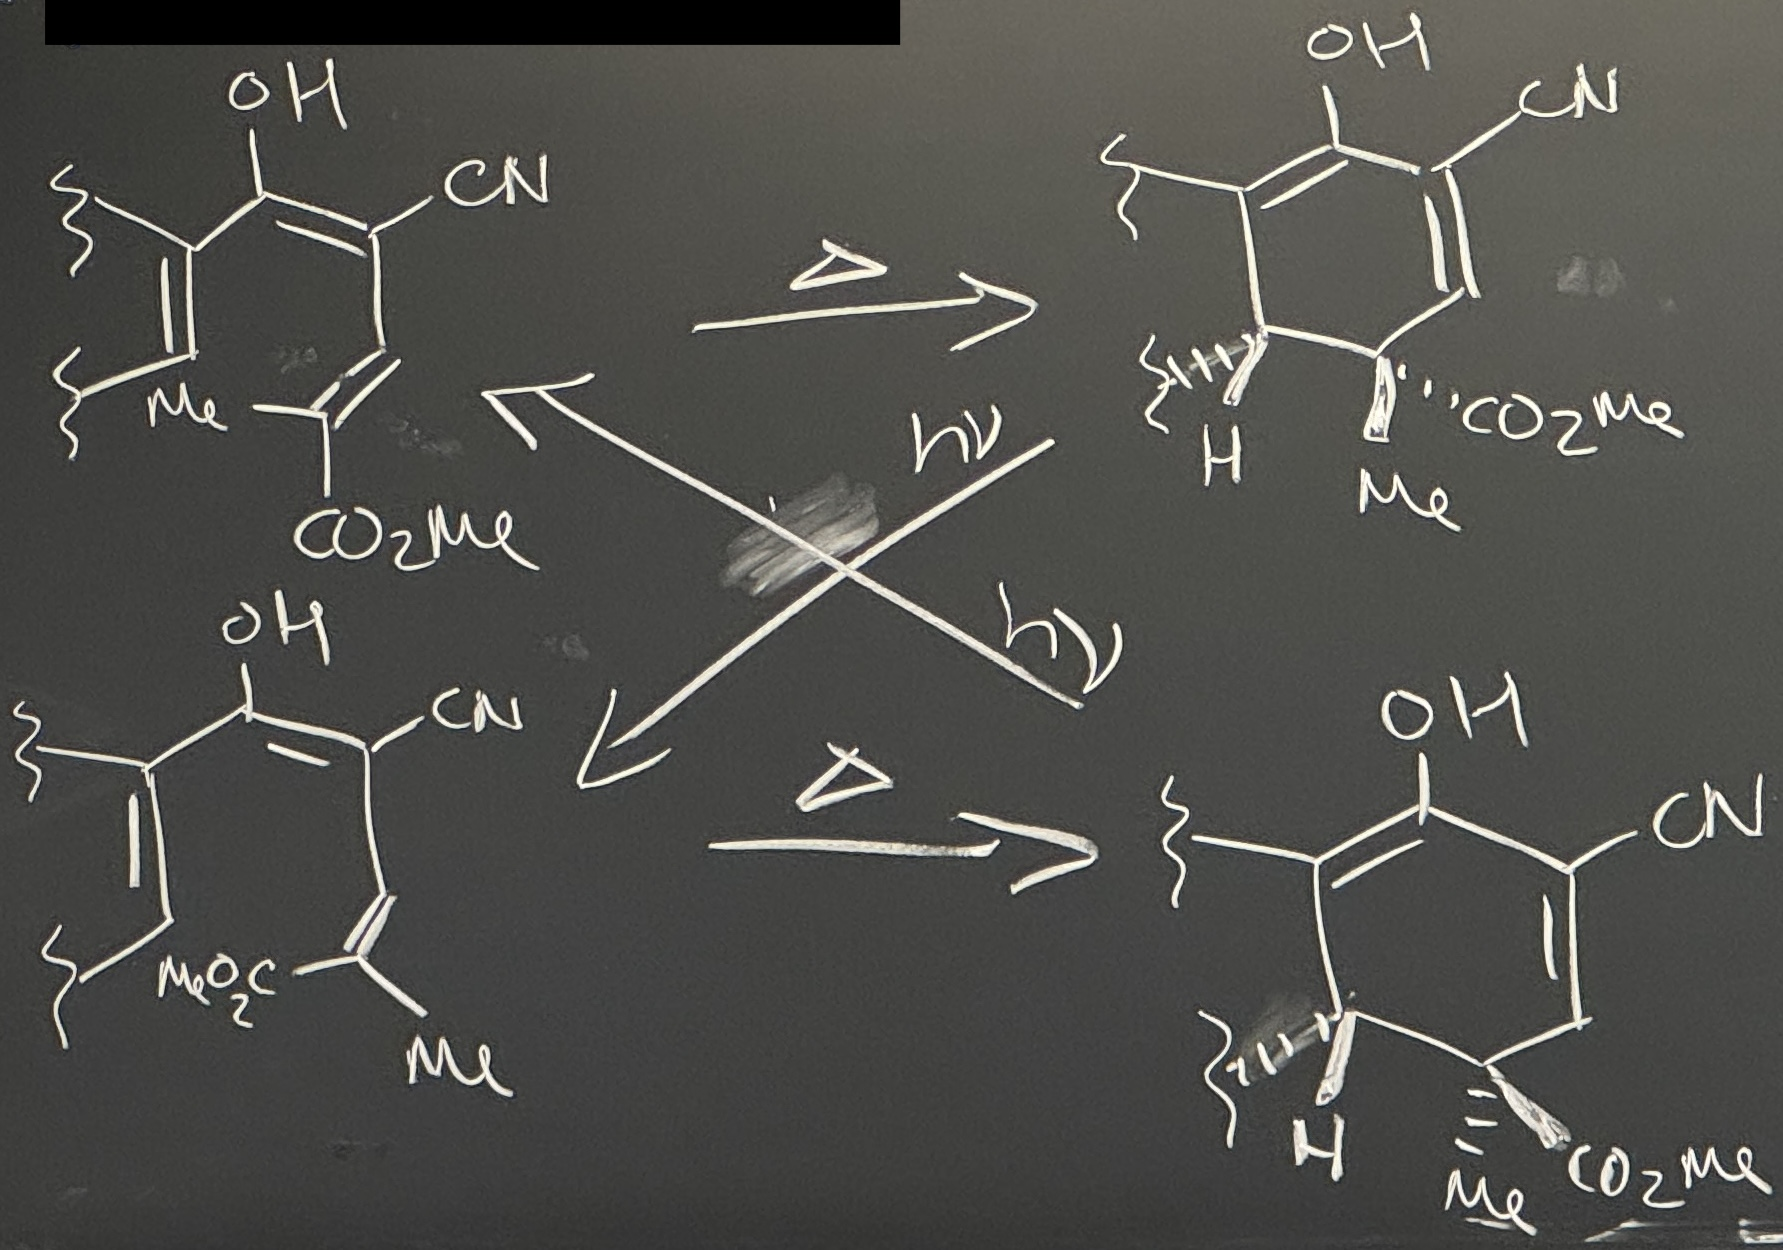
\includegraphics[width=0.4\linewidth]{woodwardB12.JPG}
        \caption{First observation of a pericyclic mechanism.}
        \label{fig:woodwardB12}
    \end{figure}
    \begin{itemize}
        \item Long considered to have "no mechanism."
        \begin{itemize}
            \item This is because people saw a starting material and a product, with nothing in between.
            \item Quote from the '60s: "No-mechanism is the designation, given half in jest, half in desperation, to thermoreorganization reactions" -- \textcite{bib:thermoReorg}.
        \end{itemize}
        \item In 1966, Woodward and his army of grad students were synthesizing Vitamin B\textsubscript{12}. During one particular ring-closing `thermoreorganization' reaction, they noticed that using different geometric isomers as starting materials formed different stereoisomers as products (see Figure \ref{fig:woodwardB12}).
        \begin{itemize}
            \item This gave a hint!
            \item Shortly after, Woodward and colleagues made a second (even weirder) observation: In the presence of light, the cyclized products would revert to their starting materials, but to the \emph{opposite} geometric isomer (also see Figure \ref{fig:woodwardB12})!
        \end{itemize}
        \item These observations kickstarted a series of studies into the mechanism of such reactions.
    \end{itemize}
    \item In time, we came to classify the reaction in Figure \ref{fig:woodwardB12} as a "$6\pi$ electrocyclization," governed by the mechanism described as follows.
    \begin{figure}[h!]
        \centering
        \begin{subfigure}[b]{0.25\linewidth}
            \centering
            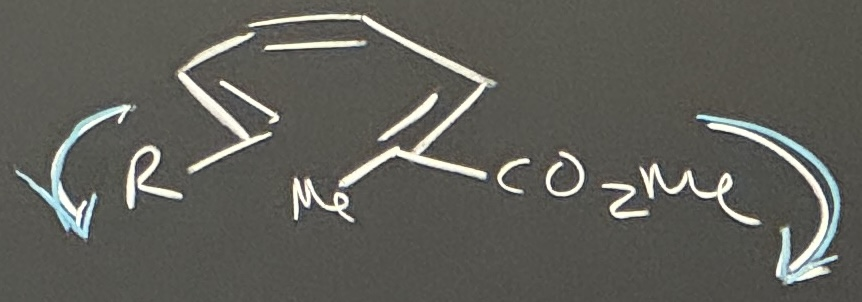
\includegraphics[width=0.9\linewidth]{disCona.JPG}
            \caption{Disrotatory.}
            \label{fig:disCona}
        \end{subfigure}
        \begin{subfigure}[b]{0.25\linewidth}
            \centering
            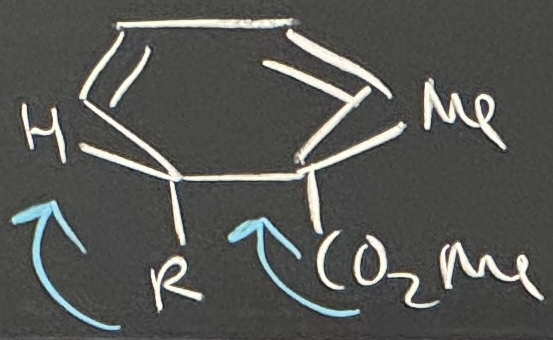
\includegraphics[width=0.6\linewidth]{disConb.JPG}
            \caption{Conrotatory.}
            \label{fig:disConb}
        \end{subfigure}
        \caption{$6\pi$ electrocyclization mechanisms.}
        \label{fig:disCon}
    \end{figure}
    \pagebreak
    \begin{itemize}
        \item During a \textbf{thermal} electrocyclization, the termini of the $\pi$-systems rotate in opposite directions.
        \begin{itemize}
            \item Notice how in Figure \ref{fig:disCona}, both \emph{exo} groups rotate down, but the right one rotates clockwise and the left one rotates clockwise.
        \end{itemize}
        \item During a \textbf{photochemical} electrocyclization, the termini of the $\pi$-system rotate in the same direction.
        \begin{itemize}
            \item Notice how in Figure \ref{fig:disConb}, both axial groups rotate clockwise.
        \end{itemize}
        \item This "rotation" of the $\pi$-systems' termini is classified as \textbf{disrotatory} and \textbf{conrotatory}, respectively.
        \begin{itemize}
            \item The disrotatory/conrotatory phenomenon led us to the \textbf{Woodward-Hoffmann rules}.
        \end{itemize}
        \item The fact that Woodward and colleagues' forward reaction is thermal but reverse reaction is photochemical is what yields the opposite starting material!
    \end{itemize}
    \item \textbf{Thermal} (reaction): A reaction driven by high temperatures.
    \item \textbf{Photochemical} (reaction): A reaction driven by light.
    \item \textbf{Disrotatory} (electrocyclic reaction): An electrocyclic reaction in which the termini of the $\pi$-systems rotate in opposite directions.
    \item \textbf{Conrotatory} (electrocyclic reaction): An electrocyclic reaction in which the termini of the $\pi$-systems rotate in the same direction.
    \item \textbf{Woodward-Hoffmann rules}: Pericyclic reactions occur by the conservation of orbital symmetry from starting material to product.
    \begin{table}[h!]
        \centering
        \small
        \renewcommand{\arraystretch}{1.2}
        \begin{tabular}{ccc}
            \textbf{Activation} & \textbf{\#\,e\textsuperscript{$\bm{-}$}} & \textbf{Rotation}\\
            \hline
            $\Delta$ & $4n$ & con\\
            $\Delta$ & $4n+2$ & dis\\
            $h\nu$ & $4n$ & dis\\
            $h\nu$ & $4n+2$ & con\\
        \end{tabular}
        \caption{Woodward-Hoffmann rules.}
        \label{tab:WHrules}
    \end{table}
    \begin{itemize}
        \item These rules are important because they allows us to predict the stereochemistry of our products.
        \item Nobel prize (1981) to Hoffmann and Fukui.
        \begin{itemize}
            \item Fukui was jointly awarded this prize for his work on frontier molecular orbital theory, which we'll talk about later in this lecture.
            \item Woodward didn't win because he had died. It was ok, though, because he had already won the Nobel once; this would have been his second.
            \item Aside (chemis-tea): A spat over who invented the Woodward-Hoffmann rules.
            \begin{itemize}
                \item E. J. Corey claimed credit for giving Woodward the idea for the Woodward-Hoffmann rules in 2004 --- see \textcite{bib:WHcorey}.
                \item Then Hoffmann rebuts Corey with a show-me-the-receipts type article --- see \textcite{bib:WHhoffmann}.
                \item Woodward and Corey were both titans in their field at Harvard, both Nobel laureates, but also both big personalities.
            \end{itemize}
            \item Aside: Anyone who believes that science is somehow unbaised and empirical has never worked with a real scientist. Masha: "Scientists are some of the most human, emotional colleagues I've has ever worked with\dots and I love them, don't get me wrong."
        \end{itemize}
        \item Historical impact: One of the first successful unions of theory and experiment in chemistry.
        \begin{itemize}
            \item Credited with leading organic chemists to finally accept MO theory.
        \end{itemize}
    \end{itemize}
    \item Let's now schematize the orbital machinations underlying the Woodward-Hoffmann rules.
    \item \textbf{Correlation diagram}: A method of tracking orbital symmetry from starting materials to products in an electrocyclization.
    \begin{itemize}
        \item Workflow.
        \begin{enumerate}
            \item Draw MOs.
            \item Assign symmetry ($\text{S}=\text{symmetric}$, $\text{A}=\text{antisymmetric}$).
            \item Populate with electrons.
            \item Correlate orbitals with the same symmetry.
        \end{enumerate}
        \item We assign symmetry differently depending on whether we're investigating a disrotatory or conrotatory pathway.
        \begin{itemize}
            \item Disrotatory pathway: Ask yourself, "are the orbitals symmetric with respect to the \textbf{$\bm{\sigma}$-plane}?"
            \item Conrotatory pathway: Ask yourself, "are the orbitals symmetric with respect to the $C_2$ axis perpendicular to the $\sigma$-bond that forms in the electrocyclization and lying in the plane of the pericyclic TS?"
        \end{itemize}
        \item For clarification on what exactly this all means, we'll look at a few examples. In particular, we'll investigate the favorability of the thermal and photochemical, disrotatory and conrotatory pathways through which the $4\pi$ electrocyclization of butadiene could proceed.
    \end{itemize}
    \item \textbf{$\bm{\sigma}$-plane}: The mirror plane lying perpendicular to the $\sigma$-bond that forms in an electrocyclization.
    \item Example: The possible thermally activated, $4\pi$ electrocyclizations of butadiene.
    \begin{figure}[h!]
        \centering
        \begin{subfigure}[b]{0.4\linewidth}
            \centering
            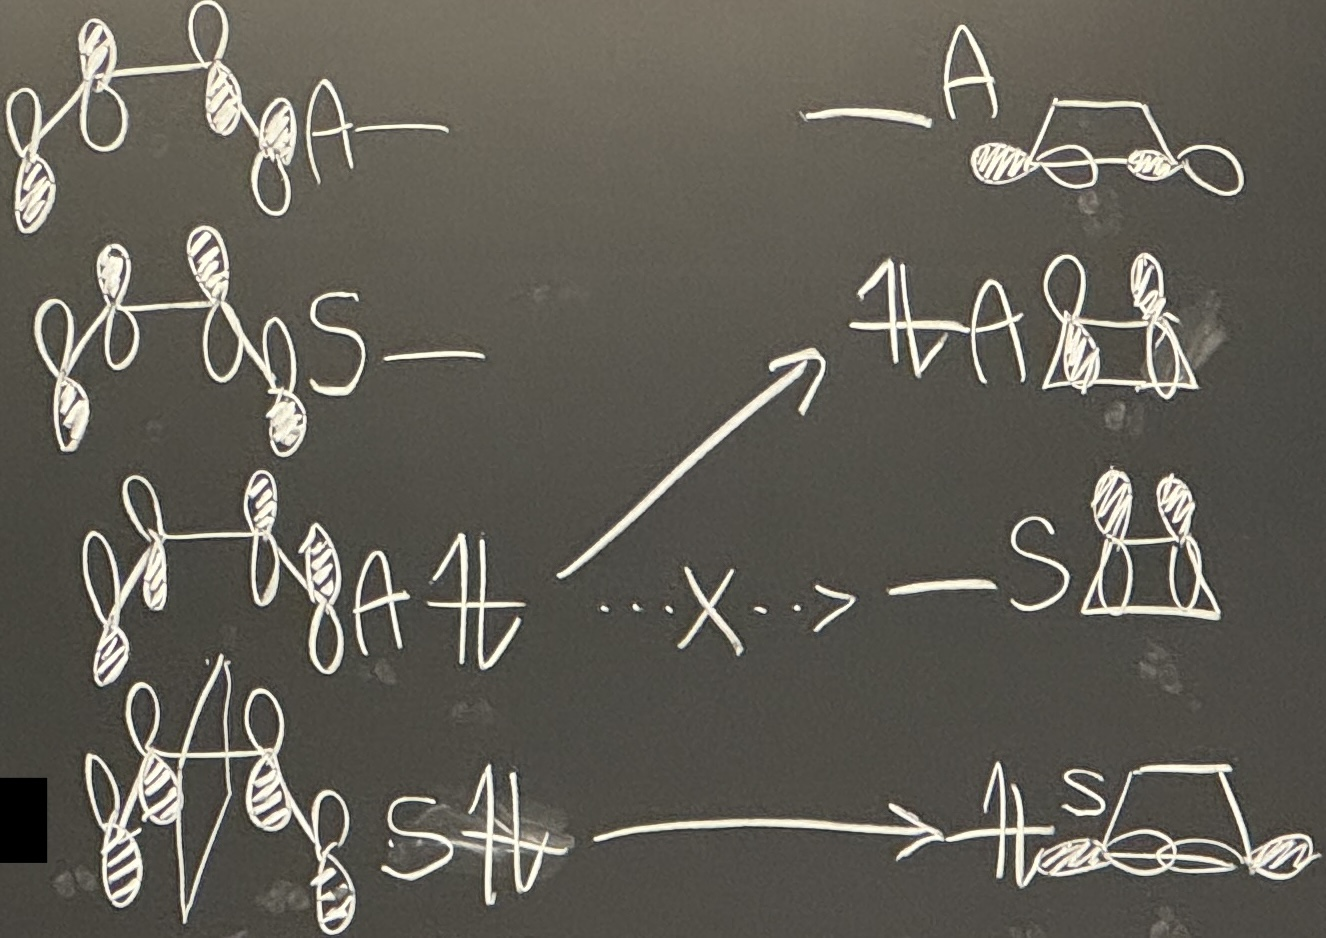
\includegraphics[width=0.8\linewidth]{4pButaTa.JPG}
            \caption{Disrotatory.}
            \label{fig:4pButaTa}
        \end{subfigure}
        \begin{subfigure}[b]{0.222\linewidth}
            \centering
            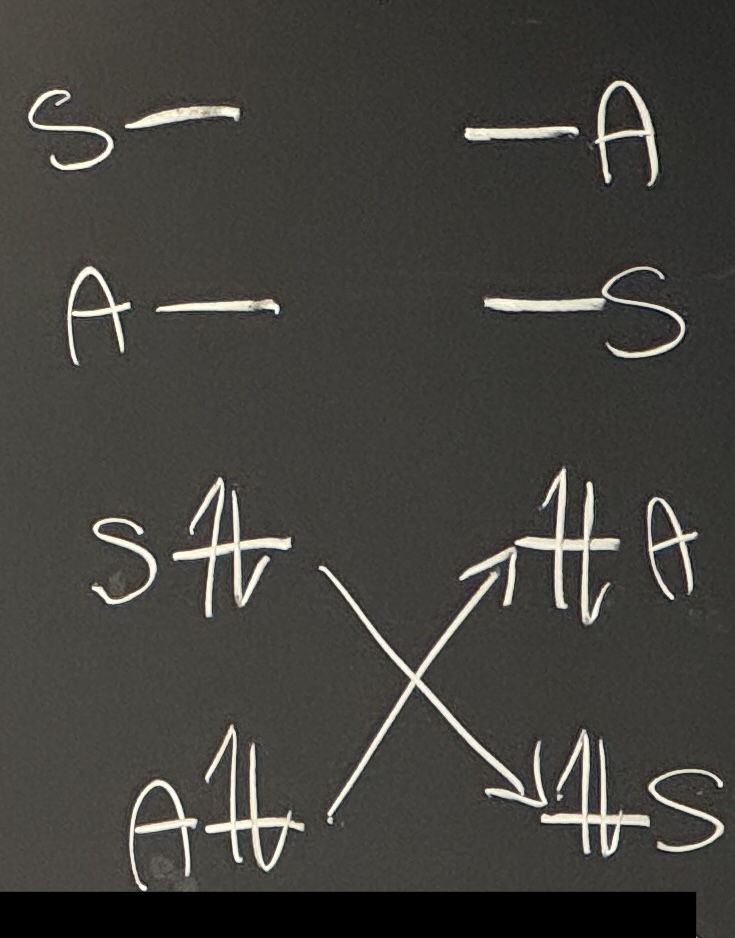
\includegraphics[width=0.8\linewidth]{4pButaTb.JPG}
            \caption{Conrotatory.}
            \label{fig:4pButaTb}
        \end{subfigure}
        \caption{Correlation diagrams for butadiene's thermal $4\pi$ electrocyclizations.}
        \label{fig:4pButaT}
    \end{figure}
    \begin{itemize}
        \item We will first apply the correlation diagram workflow to the disrotatory case (Figure \ref{fig:4pButaTa}).
        \begin{enumerate}
            \item Draw MOs for both the starting material and product.
            \begin{itemize}
                \item Let's begin by drawing the MOs for the starting material.
                \begin{itemize}
                    \item We'll draw four $p$-orbitals and shade them in to create a conjugated $\pi$-system exactly as in Huckel theory.
                    \item Specifically, notice the no nodes $\to$ 1 node $\to$ 2 nodes $\to$ 3 nodes pattern.
                \end{itemize}
                \item Then we draw the product's MOs adjacent.
                \begin{itemize}
                    \item We know that the original four $p$-orbitals are transforming into a new $\sigma$-bond and a new $\pi$-bond, so we draw the bonding and antibonding phases of the new $\sigma$-bond as well as the bonding and antibonding phases of the new $\pi$-bond.
                    \item Essentially, we are drawing a $\sigma$, $\pi$, $\pi^*$, and $\sigma^*$ MO.
                    \item Note that the $\pi$ and $\pi^*$ orbitals split less (energetically) than the $\sigma$ and $\sigma^*$ orbitals --- just like in IChem --- because they have less direct overlap; this is why we get the ordering $\sigma\to\pi\to\pi^*\to\sigma^*$ as opposed to $\pi\to\sigma\to\sigma^*\to\pi^*$ or something like that.
                \end{itemize}
            \end{itemize}
            \item Assign symmetry to each of our drawn MOs.
            \begin{itemize}
                \item Since we are looking at the \emph{disrotatory} case, we will look at symmetry with respect to the $\sigma$-plane.
                \item As a guide, we draw in the $\sigma$-plane in the bottom-left MO.
                \item This particular MO is clearly symmetric with respect to the $\sigma$-plane, so we label it "S".
                \item We then perform this analysis for the remaining MOs, noting them as either symmetric or antisymmetric.
            \end{itemize}
            \item Populate the starting MOs with electrons.
            \begin{itemize}
                \item $4\pi$ electrocyclization, so 4 electrons to fill normally (i.e., per Aufbau, Pauli, and Hund).
            \end{itemize}
            \item Correlate the filled starting MOs to the lowest energy product MOs with matching symmetry.
            \begin{itemize}
                \item Maxim: An orbital cannot flip its symmetry during an electrocyclization.
                \item As such, the lowest energy starting MO (being symmetric) has no problem becoming the lowest energy product MO (which is also symmetric).
                \item However, the second-lowest energy starting MO (being antisymmetric) \emph{cannot} become the second-lowest energy product MO because the latter is symmetric. (We say that this transition is formally \textbf{forbidden} because symmetry is not conserved.) As such, it must go up in energy to become the third-lowest energy product MO.
                \item This population of a higher energy orbital means that the $4\pi$ electrocyclization of butadiene is \emph{disfavored} to occur through a thermal, disrotatory pathway.
            \end{itemize}
        \end{enumerate}
        \item We now apply the correlation diagram workflow to the conrotatory case (Figure \ref{fig:4pButaTb}).
        \begin{enumerate}
            \item The MOs will be the same as in Figure \ref{fig:4pButaTa}, so we don't need to redraw them.
            \item The symmetry must be evaluated with respect to that $C_2$ axis this time, though, so we have to reassign S or A to each MO.
            \begin{itemize}
                \item For the MOs as drawn in Figure \ref{fig:4pButaTa}, the $C_2$ axis we need goes into the plane of the page.
            \end{itemize}
            \item We populate the starting MOs as before.
            \item When we correlate, this time we can fill the bottom two product MOs!
            \begin{itemize}
                \item We didn't populate electrons directly across, but we \emph{did} populate the lowest energy orbitals again, so the conrotatory pathway is \emph{favored}.
                \item Both arrows involve a conservation of orbital symmetry, so (to reiterate) this reaction is \textbf{allowed} (thermally).
            \end{itemize}
        \end{enumerate}
    \end{itemize}
    \item David: Why do we only draw some of the molecular orbitals?
    \begin{figure}[h!]
        \centering
        \footnotesize
        \schemestart
            \chemfig{*4([2]=[@{1}]-[@{2}]=[@{3}]-[@{4},,,,opacity=0])}
            \arrow{<=>}
            \chemfig{*4([2]-=--)}
        \schemestop
        \chemmove{
            \draw [curved arrow={4pt}{2pt}] (1) to[bend right=45,looseness=1.5] (4);
            \draw [curved arrow={4pt}{2pt}] (3) to[bend right=45,looseness=1.5] (2);
        }
        \caption{MOs relevant to butadiene's $4\pi$ electrocyclization.}
        \label{fig:butaElectroMOs}
    \end{figure}
    \begin{itemize}
        \item We only consider the orbitals involved in the reaction; considering the whole $\sigma$-network would get more complicated without changing our results.
        \item This is actually an example of why arrow-pushing is useful! Namely, because it shows that the $p$-MOs we consider in the starting material become the $\sigma$- and $\pi$-MOs we consider in the product.
    \end{itemize}
    \item \textbf{Photochemical reaction}: A reaction driven by the absorption of a photon, leading to an excited state.
    \begin{itemize}
        \item Later in this course, we'll go more into detail on photochemical reactions, but this is the only level of detail we need right now.
        \item In the reactions we'll look at today, one electron is kicked up an energy level with no other changes to the structure.
    \end{itemize}
    \pagebreak
    \item Example: The possible photochemically activated, $4\pi$ electrocyclizations of butadiene.
    \begin{figure}[h!]
        \centering
        \begin{subfigure}[b]{0.3\linewidth}
            \centering
            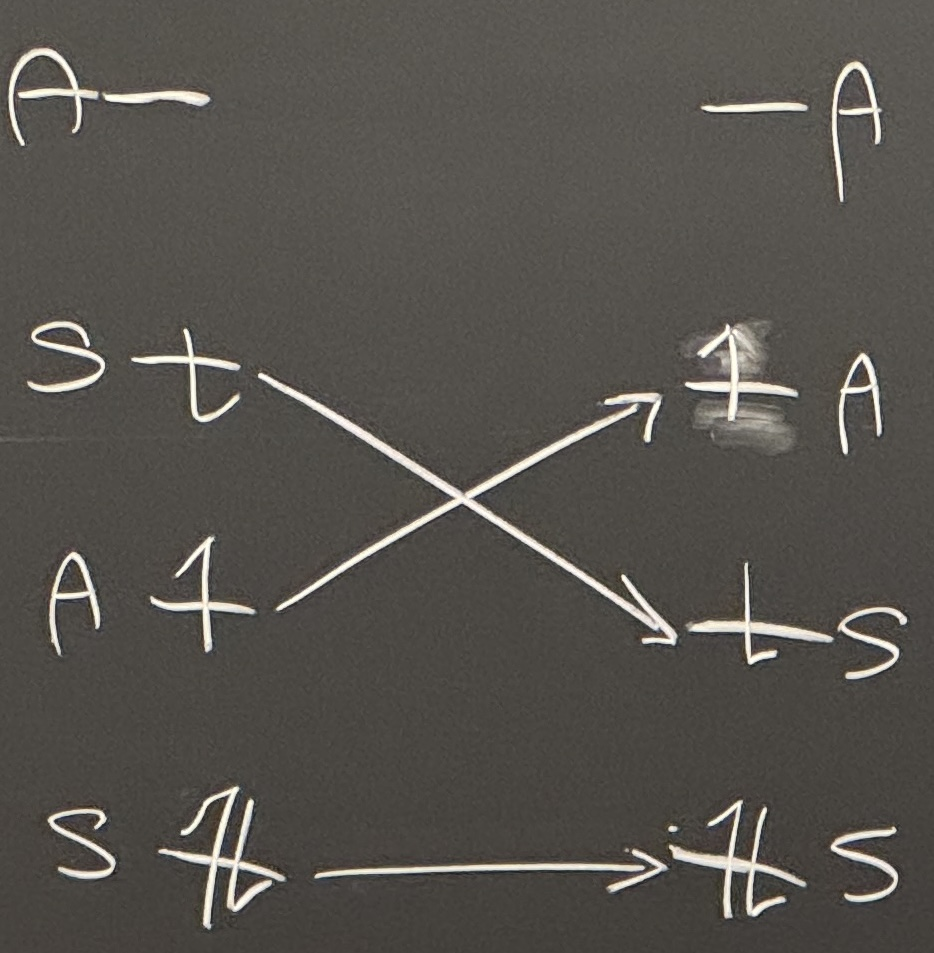
\includegraphics[width=0.8\linewidth]{4pButaPa.JPG}
            \caption{Disrotatory.}
            \label{fig:4pButaPa}
        \end{subfigure}
        \begin{subfigure}[b]{0.3\linewidth}
            \centering
            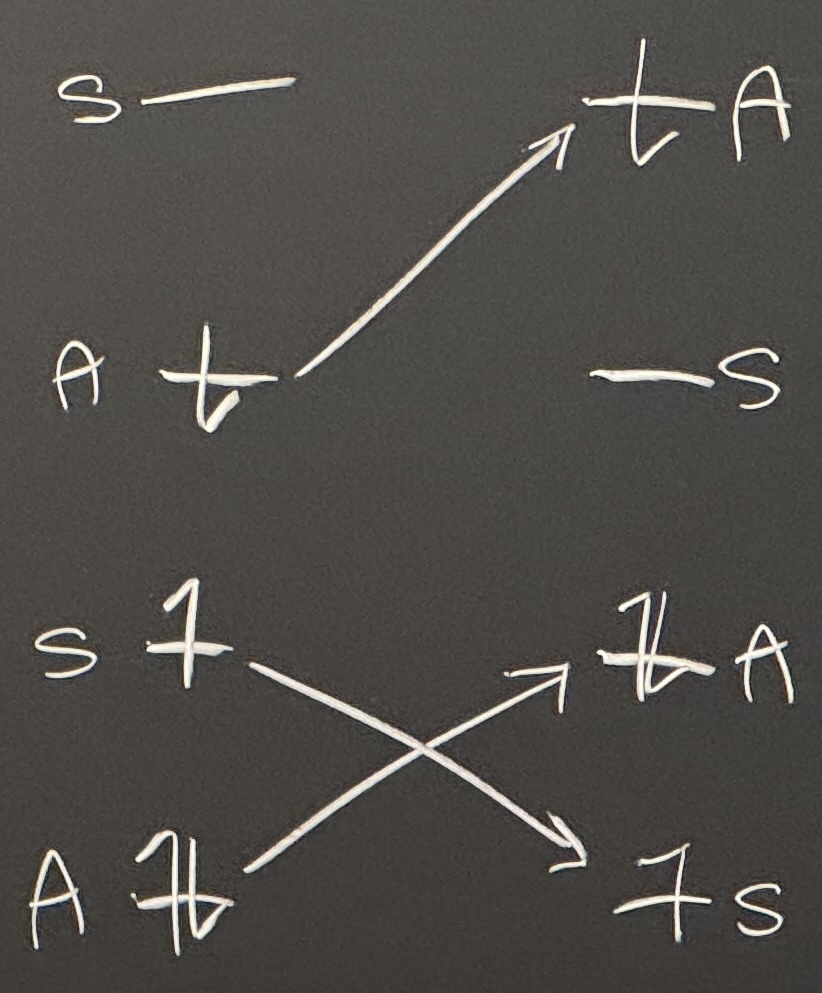
\includegraphics[width=0.68\linewidth]{4pButaPb.JPG}
            \caption{Conrotatory.}
            \label{fig:4pButaPb}
        \end{subfigure}
        \caption{Correlation diagrams for butadiene's photochemical $4\pi$ electrocyclizations.}
        \label{fig:4pButaP}
    \end{figure}
    \begin{itemize}
        \item We use the same MOs and symmetries as in the corresponding subfigures of Figure \ref{fig:4pButaT}.
        \item Differences only start to appear when we populate with electrons.
        \begin{itemize}
            \item In particular, we excite one electron up a level (without altering its spin) in both sets of starting-material MOs.\footnote{I.e., without intersystem crossing to a triplet state.}
        \end{itemize}
        \item Disrotatory case (Figure \ref{fig:4pButaPa}).
        \begin{itemize}
            \item Orbital symmetries are such that we end up with the \emph{same} populations as in the starting material.
            \item Therefore, this pathway is allowed/favored.
        \end{itemize}
        \item Conrotatory case (Figure \ref{fig:4pButaPb}).
        \begin{itemize}
            \item Orbital symmetries are such that we end up with a \emph{higher-energy} population than in the starting material.
            \item Since electrons are in "much higher" energy levels, this pathway is forbidden/disfavored.
        \end{itemize}
    \end{itemize}
    \item Notice that the photochemical result that disrotatory is favored and conrotatory is disfavored is the opposite of thermal!
    \begin{itemize}
        \item Thus, we just derived the Woodward-Hoffmann rules (Table \ref{tab:WHrules}) about what is favored and disfavored!
        \begin{itemize}
            \item At least we derived the case for 4 electrons.
            \item A more general mathematical proof can be done to rigorously verify Table \ref{tab:WHrules}, but the details are beyond the scope of this class.
        \end{itemize}
        \item If you ever forget the WH rules, just rederive them from first principles :)
    \end{itemize}
    \item A note on the correlation arrows in Figures \ref{fig:4pButaT} and \ref{fig:4pButaP}.
    \begin{itemize}
        \item The uppermost correlation arrow in Figure \ref{fig:4pButaPb} corresponds to an \emph{allowed} but \emph{disfavored} electronic transition.
        \item The X'ed-out correlation arrow from A to S in Figure \ref{fig:4pButaTa} corresponds to an explicitly \emph{forbidden} electronic transition.
    \end{itemize}
    \item The Woodward-Hoffmann rules are one way to look at pericyclic reactions, probably the most complex way.
    \begin{itemize}
        \item We'll now look at two simpler ways.
    \end{itemize}
    \item Dewar-Zimmerman analysis: Aromatic TS theory.
    \begin{itemize}
        \item Principle: Reactions that go through aromatic transition states are allowed.
        \item We already like 6-membered TS's because they're geometrically stable; 6-membered \emph{aromatic} TS's are even lower energy and more favored!
    \end{itemize}
    \item Examples of aromatic and antiaromatic transition states.
    \begin{figure}[h!]
        \centering
        \begin{subfigure}[b]{0.5\linewidth}
            \centering
            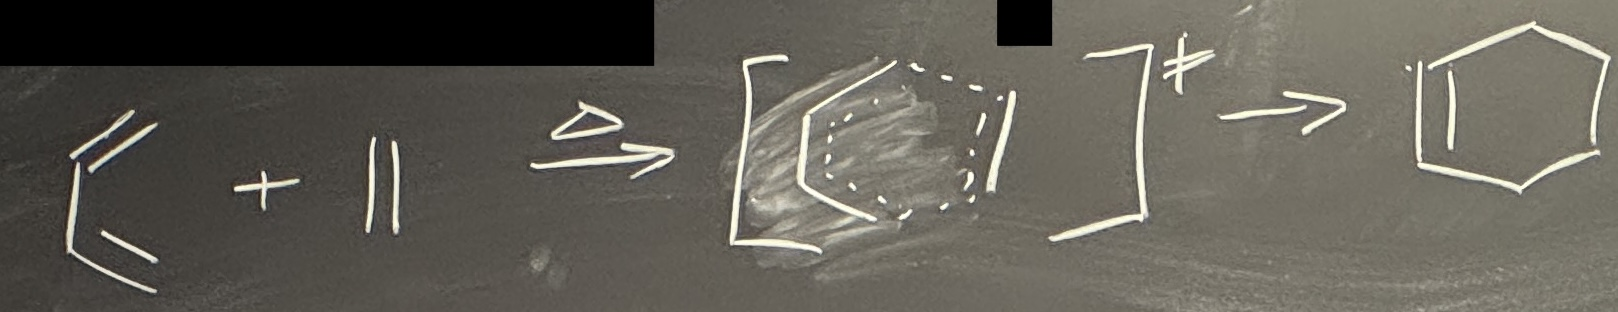
\includegraphics[width=0.9\linewidth]{DZarAntia.JPG}
            \caption{Aromatic TS in a $[4+2]$ cycloaddition.}
            \label{fig:DZarAntia}
        \end{subfigure}\\[2em]
        \begin{subfigure}[b]{0.5\linewidth}
            \centering
            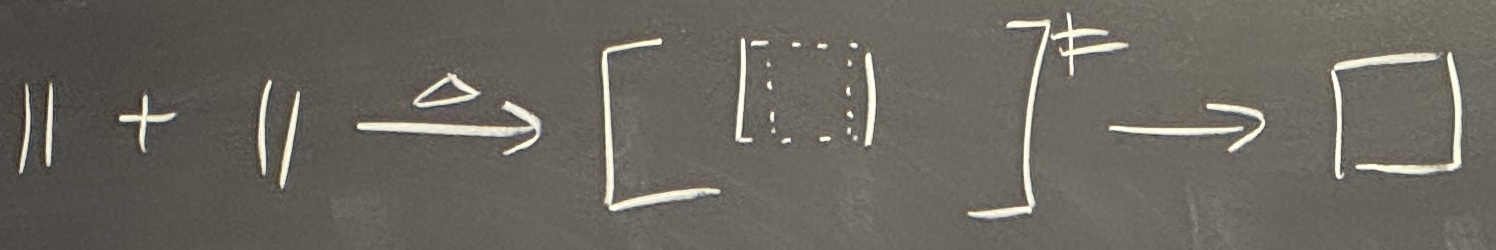
\includegraphics[width=0.9\linewidth]{DZarAntib.JPG}
            \caption{Anitaromatic TS in a $[2+2]$ cycloaddition.}
            \label{fig:DZarAntib}
        \end{subfigure}
        \caption{Aromatic and antiaromatic transition states.}
        \label{fig:DZarAnti}
    \end{figure}
    \begin{itemize}
        \item Figure \ref{fig:DZarAntia} shows that the transition state in a Diels-Alder reaction is aromatic.
        \begin{itemize}
            \item This is why the forward Diels-Alder reaction is favored (under thermal conditions).
        \end{itemize}
        \item Figure \ref{fig:DZarAntib} shows that the transition state in a $[2+2]$ cycloaddition is antiaromatic.
        \begin{itemize}
            \item This is why the forward reaction to cyclobutane is disfavored (under thermal conditions).
        \end{itemize}
    \end{itemize}
    \item Let's get a little more formal now.
    \item Rules.
    \begin{enumerate}
        \item Draw orbitals with any phasing, and decide the reaction topology.
        \begin{itemize}
            \item By "any phasing," we do mean that you can take \emph{any} of the MOs you would draw and the Dewar-Zimmerman analysis will still work. So "go crazy," if you want!
            \begin{itemize}
                \item Masha does not draw out any examples to inductively prove this to us, but it would probably be a good exercise to do this on my own!!
            \end{itemize}
            \item By "reaction topology," we mean how the two reactants approach each other. Is something coming from the top? The bottom?
        \end{itemize}
        \item Connect orbitals through the reaction topology and count the number of phase inversions (PIs).
        \begin{itemize}
            \item In other words, count how many lines connect lobes of opposite phases.
            \item This will tell us whether we should evaluate the transition state for \emph{Huckel} or \emph{M\"{o}bius} aromaticity.
            \item Essentially\dots
            \begin{itemize}
                \item If there are an \emph{even} number of PIs, having $4n+2$ electrons will lend \emph{Huckel} aromaticity to the transition state and favor its formation;
                \item If there are an \emph{odd} number of PIs, having $4n$ electrons will lend \emph{M\"{o}bius} aromaticity to the transition state and favor its formation.
            \end{itemize}
        \end{itemize}
        \item Count the number of electrons.
        \begin{itemize}
            \item As mentioned above, this number will tell us (depending on whether we're in Huckel-land or M\"{o}bius-land) whether the transition state is aromatic.
        \end{itemize}
    \end{enumerate}
    \pagebreak
    \item To practice using these rules, let's reevaluate the examples in Figure \ref{fig:DZarAnti}.
    \begin{figure}[h!]
        \centering
        \begin{subfigure}[b]{0.17\linewidth}
            \centering
            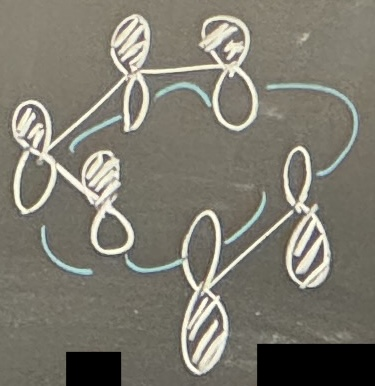
\includegraphics[width=0.68\linewidth]{DZrulesa.JPG}
            \caption{$[4+2]$.}
            \label{fig:DZrulesa}
        \end{subfigure}
        \begin{subfigure}[b]{0.17\linewidth}
            \centering
            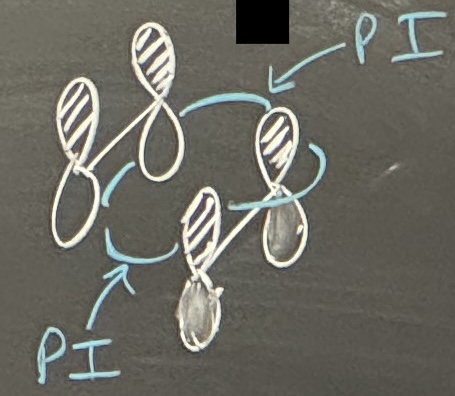
\includegraphics[width=0.8\linewidth]{DZrulesb.JPG}
            \caption{$[2+2]$.}
            \label{fig:DZrulesb}
        \end{subfigure}
        \caption{Dewar-Zimmerman connections for $[4+2]$ and $[2+2]$ cycloadditions.}
        \label{fig:DZrules}
    \end{figure}
    \begin{itemize}
        \item Example: $[4+2]$ cycloaddition (Figure \ref{fig:DZrulesa}).
        \begin{enumerate}
            \item Draw MOs, and decide the reaction topology.
            \begin{itemize}
                \item MOs: Let's arbitrarily choose to use the MOs with no nodes for both butadiene and ethene.
                \item Topology: Let ethene approach butadiene from the bottom.
            \end{itemize}
            \item Connect orbitals, and count PIs.
            \begin{itemize}
                \item Connections: We connect all the bottom lobes of butadiene, the two top lobes of ethene, and (since ethene is approaching from the bottom, per the reaction topology) the bottom terminal lobes of butadiene to the top terminal lobes of ethene.
                \begin{itemize}
                    \item The connections are all drawn as blue lines in Figure \ref{fig:DZrules}.
                \end{itemize}
                \item PIs: All of the connected lobes are unshaded, so there are 0 PIs.
                \item 0 is an even number, so we are in Huckel-land.
            \end{itemize}
            \item Count the number of electrons.
            \begin{itemize}
                \item There are $6=4(1)+2$ $\pi$-electrons.
                \item Therefore, our TS will be \emph{stabilized} by \emph{aromaticity} of the \emph{Huckel} type.
            \end{itemize}
        \end{enumerate}
        \item Example: $[2+2]$ cycloaddition (Figure \ref{fig:DZrulesb}).
        \begin{enumerate}
            \item Draw MOs, and decide the reaction topology.
            \begin{itemize}
                \item MOs: We once again choose (arbitrarily) the MOs with no nodes for both ethenes.
                \item Topology: The right ethene approaches the left ethene from the bottom.
            \end{itemize}
            \item Connect orbitals, and count PIs.
            \begin{itemize}
                \item Connections: We connect the bottom lobes of the left ethene to each other and to the top lobes of the right ethene (which are also connected to each other).
                \item PIs: This time --- because of the way we have drawn the right ethene --- we have 2 PIs.
                \item 2 is an even number, so we are in Huckel-land.
            \end{itemize}
            \item Count the number of electrons.
            \begin{itemize}
                \item There are $4=4(1)$ $\pi$-electrons.
                \item Therefore, our TS will be \emph{destabilized} by \emph{antiaromaticity} of the \emph{Huckel} type.
            \end{itemize}
        \end{enumerate}
    \end{itemize}
    \item The Dewar-Zimmerman analysis is useful for predicting the feasibility of sigmatropic rearrangements.
    \begin{itemize}
        \item Recall from above that a \emph{sigmatropic rearrangement} involves the migration of a $\sigma$-bond along with a corresponding reorganization of the $\pi$-electrons.
        \item Specifically, in a sigmatropic rearrangement, the total number of $\pi$- and $\sigma$-bonds does not change.
    \end{itemize}
    \item Example sigmatropic rearrangements.
    \begin{enumerate}
        \item \textbf{Claisen rearrangement}.
        \item \textbf{Cope rearrangement}.
    \end{enumerate}
    \item \textbf{Claisen rearrangement}: A $[3,3]$-sigmatropic rearrangement of allyl vinyl ethers to form corresponding $\gamma,\delta$-unsaturated carbonyls.
    \begin{center}
        \footnotesize
        \setchemfig{atom sep=1.4em}
        \schemestart
            \chemfig{*6([4]=-O--=)}
            \arrow{<=>}
            \chemfig{*6(=---=O)}
        \schemestop
    \end{center}
    \item \textbf{Cope rearrangement}: A $[3,3]$-sigmatropic rearrangement of $1,5$-dienes to form other $1,5$-dienes.
    \begin{center}
        \footnotesize
        \setchemfig{atom sep=1.4em}
        \schemestart
            \chemfig{*6([4]=---=)}
            \arrow{<=>}
            \chemfig{*6(=---=)}
        \schemestop
    \end{center}
    \item We should be familiar with both the Claisen and Cope rearrangements; if we're not, Google them!!
    \item Example: Dewar-Zimmerman analysis of \textbf{suprafacial} and \textbf{antarafacial} [1,3]-sigmatropic \ce{H} shifts.
    \begin{figure}[h!]
        \centering
        \begin{subfigure}[b]{0.41\linewidth}
            \centering
            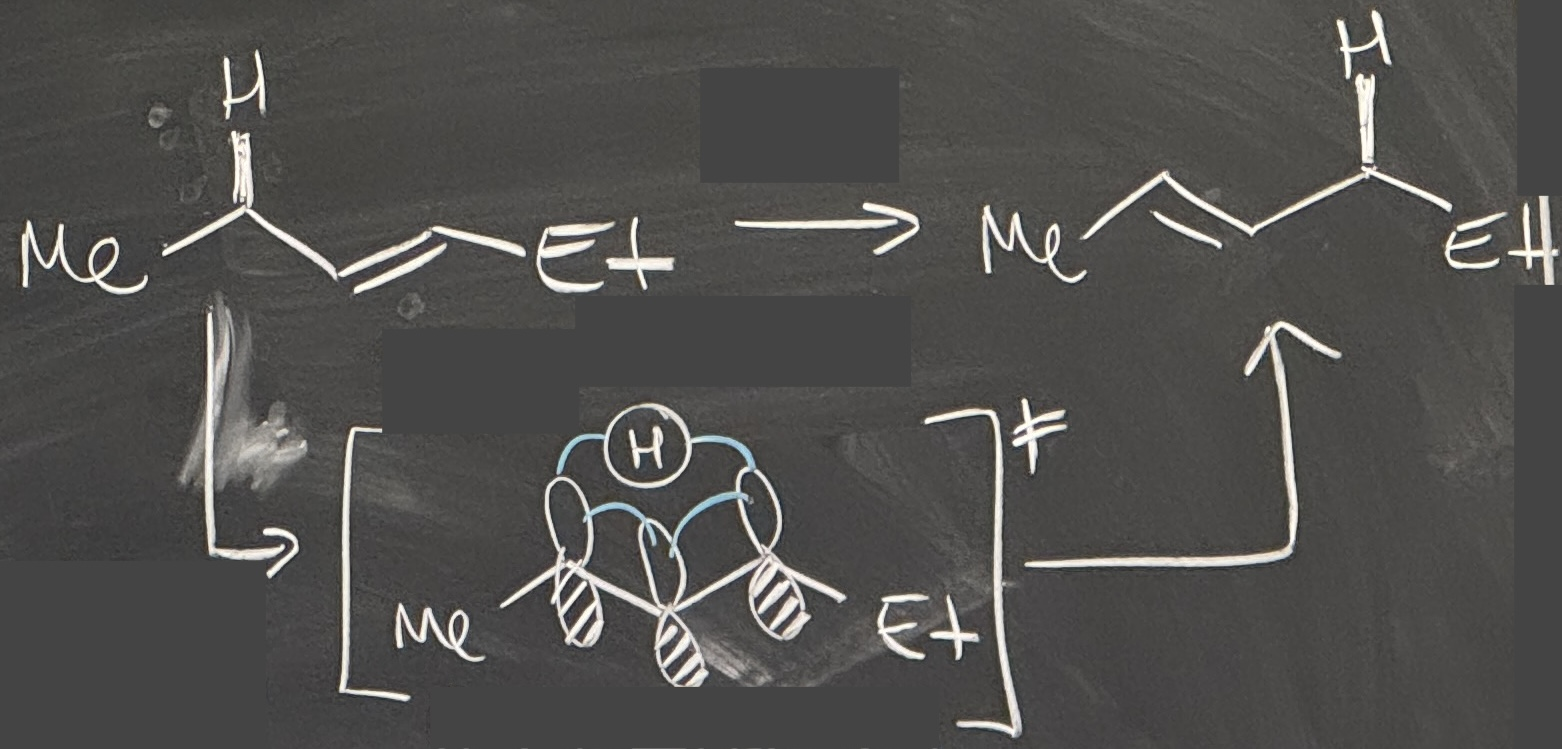
\includegraphics[width=0.9\linewidth]{supraAntaraa.JPG}
            \caption{Suprafacial.}
            \label{fig:supraAntaraa}
        \end{subfigure}
        \begin{subfigure}[b]{0.35\linewidth}
            \centering
            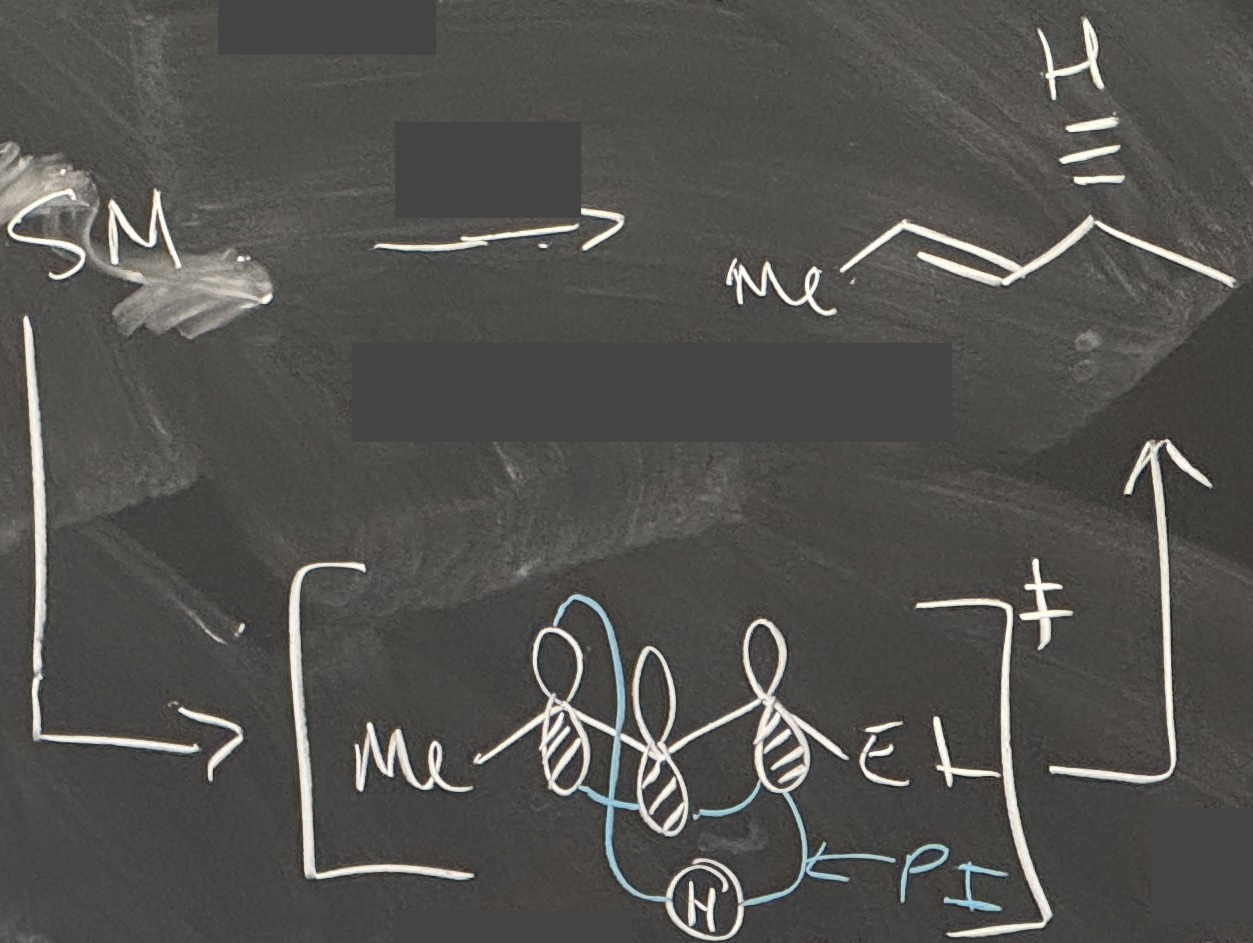
\includegraphics[width=0.8\linewidth]{supraAntarab.JPG}
            \caption{Antarafacial.}
            \label{fig:supraAntarab}
        \end{subfigure}
        \caption{Dewar-Zimmerman analysis of $[1,3]$-sigmatropic hydride shifts.}
        \label{fig:supraAntara}
    \end{figure}
    \begin{itemize}
        \item We'll start with the suprafacial case (Figure \ref{fig:supraAntaraa}).
        \begin{enumerate}
            \item Draw MOs, and decide the reaction topology.
            \begin{itemize}
                \item MOs: We choose the MO with no nodes for the $\pi$ bonds, and the hydrogen atom's $1s$ orbital.
                \begin{itemize}
                    \item Notice that we draw a $p$-orbital for all three carbons involved in the bond breaking/making process in the transition state, not just the two carbons involved in the initial or final bond!
                \end{itemize}
                \item Topology: Draw the \ce{H} atom in the process of migrating.
            \end{itemize}
            \item Connect orbitals, and count PIs.
            \begin{itemize}
                \item Connections: Connect all the top lobes together and to hydrogen.
                \item PIs: 0.
                \item Even PIs, hence Huckel.
            \end{itemize}
            \item Count the number of electrons.
            \begin{itemize}
                \item We have two electrons in the \ce{C=C} $\pi$-bond, and two electrons in the \ce{C-H} $\sigma$-bond.
                \begin{itemize}
                    \item We also get a clue that there are 4 electrons present because we drew 4 orbitals!
                \end{itemize}
                \item Thus, there are $4=4(1)$ electrons present.
                \item Therefore, our TS will be destabilized by Huckel antiaromaticity.
                \item It follows that the suprafacial pathway is (thermally) forbidden.
                \begin{itemize}
                    \item This is an interesting result because at first glance, it "looks" like a nice TS (with the H just bouncing over), but nope! It's not allowed.
                \end{itemize}
            \end{itemize}
        \end{enumerate}
        \pagebreak
        \item We now move onto the antarafacial case (Figure \ref{fig:supraAntarab}).
        \begin{enumerate}
            \item Draw MOs, and decide the reaction topology.
            \begin{itemize}
                \item MOs: Same as in Figure \ref{fig:supraAntaraa}.
                \item Topology: The \ce{H} atom is switching faces, so it will have to engage with the top lobe on one side and the bottom lobe on the other side.
            \end{itemize}
            \item Connect orbitals, and count PIs.
            \begin{itemize}
                \item Connections: We connect the three $p$-orbitals as expected, but note the explicit connection of the top-left $p$-lobe and the bottom-right $p$-lobe to the hydrogen, in accordance with the reaction topology.
                \begin{itemize}
                    \item Note that it doesn't really matter which lobes of the $p$-orbitals we connect because we get the same result either way.
                \end{itemize}
                \item PIs: 1.
                \item This is our first time having an \emph{odd} number of PIs, so we are now in M\"{o}bius-land!
            \end{itemize}
            \item Count the number of electrons.
            \begin{itemize}
                \item As above, there are $4=4(1)$ electrons.
                \item However, because we are in M\"{o}bius-land, this nevertheless means that our TS will be \emph{stabilized} by \emph{aromaticity} of the \emph{M\"{o}bius} type.
                \item Thus, "ugly" antarafacial transition states are nevertheless totally allowed!
            \end{itemize}
        \end{enumerate}
        \item Despite the fact that antarafacial $[1,3]$-sigmatropic hydride shifts are favored over their suprafacial counterparts, our intuition that the antarafacial transition state would be sterically strained is correct.
        \begin{itemize}
            \item Indeed, there are examples of $[1,3]$-hydride shifts occurring with stereoinversion, but they are rare.
            \item Nevertheless, this is a fun and nonintuitive finding!
            \item If you are interested, you can look into work on antarafacial $[1,3]$-methyl shifts, which are also favored over their suprafacial counterparts!
        \end{itemize}
        \item Aside: One place where we do see stereoinversions.
        \begin{itemize}
            \item The keto-enol tautomerization could be thought of as a $[1,3]$-sigmatropic hydride shift!
            \item Indeed, if it occurs intramolecularly, it would occur with stereoinversion.
            \item However, the rate of this intramolecular rearrangement is naturally very slow due to strain, which is why we need a solvent, acid, or base catalyst to do the proton transfer intermolecularly with any appreciable rate.
            \item Essentially, the reaction can't really happen intramoleuclarly because it'd be forbidden electronically with \emph{cis} hydrogens or very disfavored sterically with \emph{trans} hydrogens.
        \end{itemize}
    \end{itemize}
    \item \textbf{Suprafacial} (sigmatropic rearrangement): A sigmatropic rearrangement in which the bond-breaking and bond-making processes occur on the \emph{same} face of the $\pi$-system.
    \item \textbf{Antarafacial} (sigmatropic rearrangement): A sigmatropic rearrangement in which the bond-breaking and bond-making processes occur on \emph{opposite} faces of the $\pi$-system.
    \item Notice how\dots
    \begin{itemize}
        \item In Figure \ref{fig:supraAntaraa}, the hydride is on the same side of the molecule in both starting material and product, i.e., coming out of the plane of the page;
        \begin{itemize}
            \item That's why we call this suprafacial!
        \end{itemize}
        \item In Figure \ref{fig:supraAntarab}, the hydride is on opposite sides of the molecule in the starting material vs. the product, i.e., coming out of the plane of the page vs. going into the plane of the page.
        \begin{itemize}
            \item That's why we call this antarafacial!
        \end{itemize}
    \end{itemize}
    \pagebreak
    \item Frontier molecular orbital theory (FMO).
    \begin{itemize}
        \item By Fukui, as mentioned above.
        \item This is a simplification of some other models in which you only consider the HOMO/LUMO interactions (instead of all MOs).
        \item Principle: If the HOMO of the electron-donating species and LUMO of the electron-accepting species mix favorably, then the reaction is allowed.
    \end{itemize}
    \item Example: FMO analysis of cycloadditions.
    \begin{figure}[h!]
        \centering
        \begin{subfigure}[b]{0.3\linewidth}
            \centering
            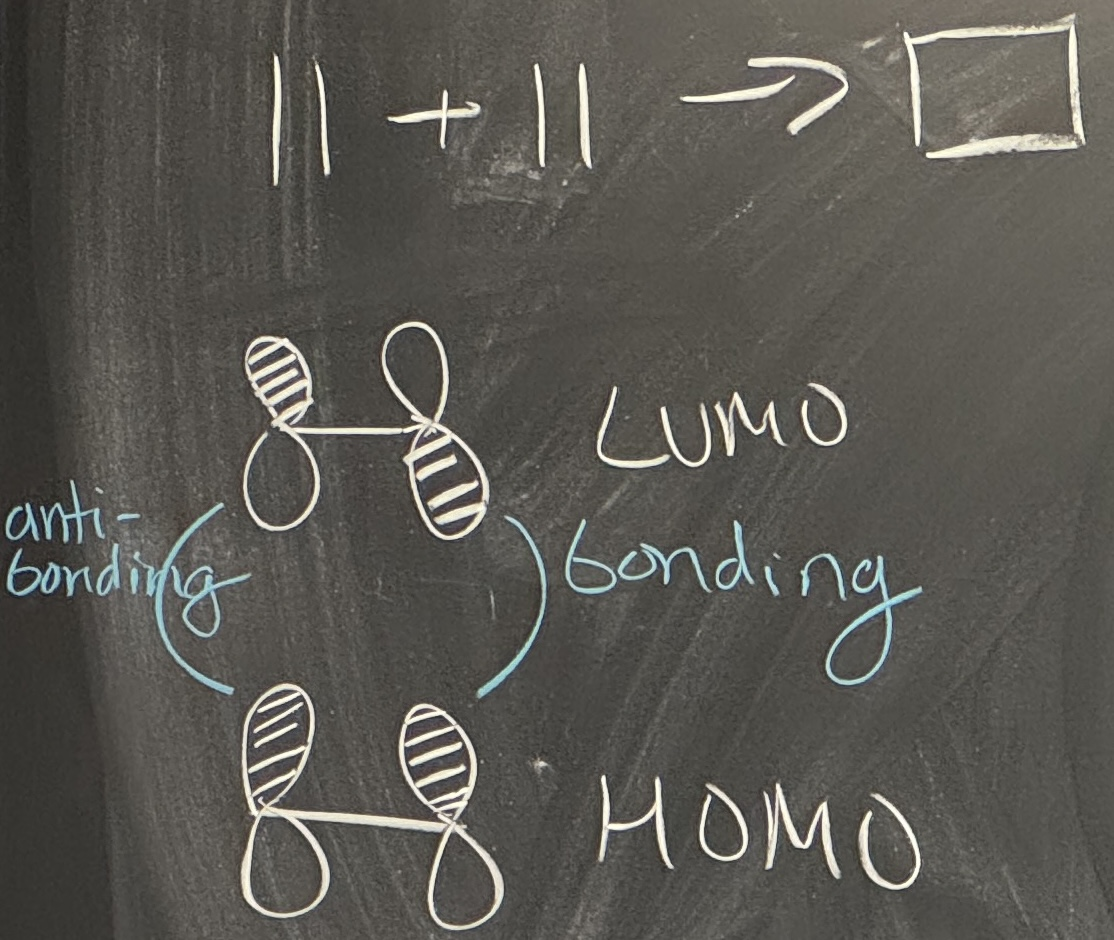
\includegraphics[width=0.8\linewidth]{FMOa.JPG}
            \caption{$[2+2]$.}
            \label{fig:FMOa}
        \end{subfigure}
        \begin{subfigure}[b]{0.3\linewidth}
            \centering
            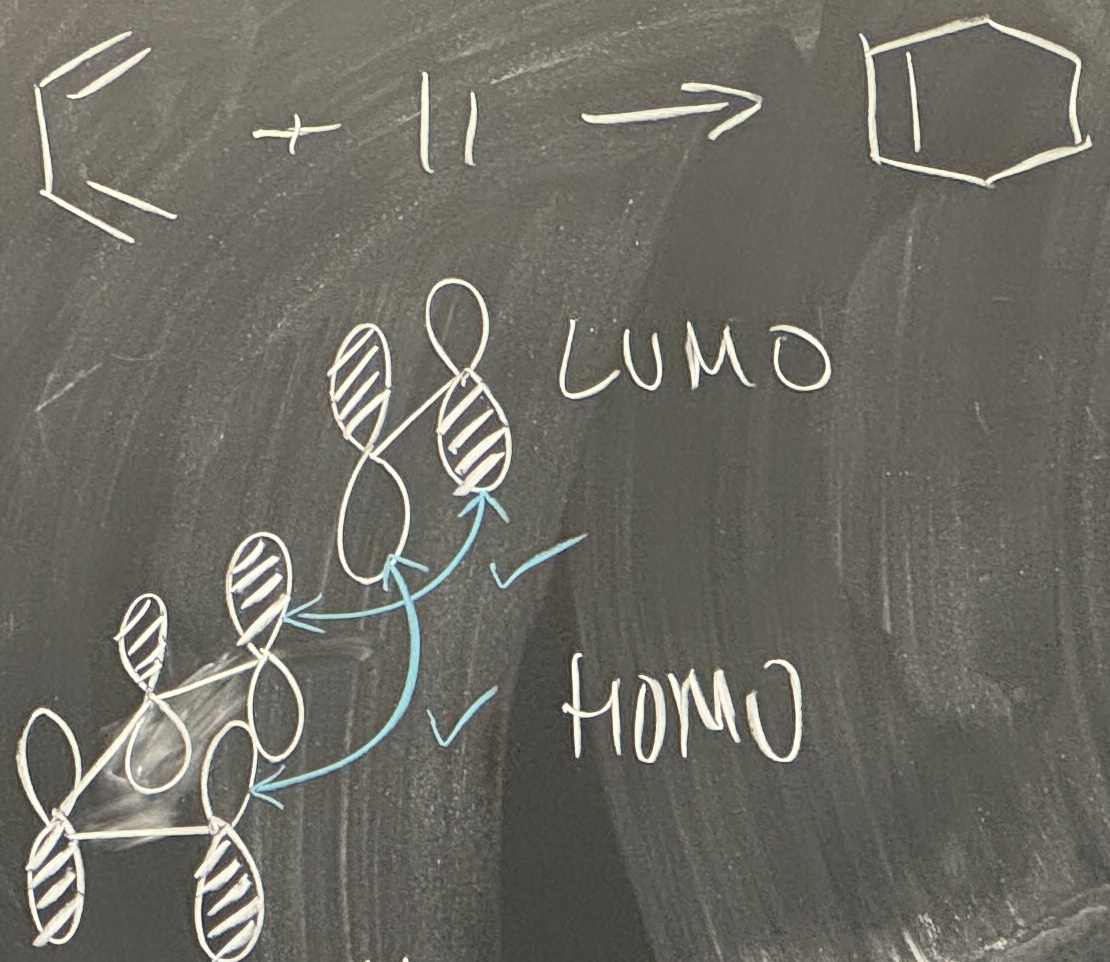
\includegraphics[width=0.78\linewidth]{FMOb.JPG}
            \caption{$[4+2]$.}
            \label{fig:FMOb}
        \end{subfigure}
        \begin{subfigure}[b]{0.3\linewidth}
            \centering
            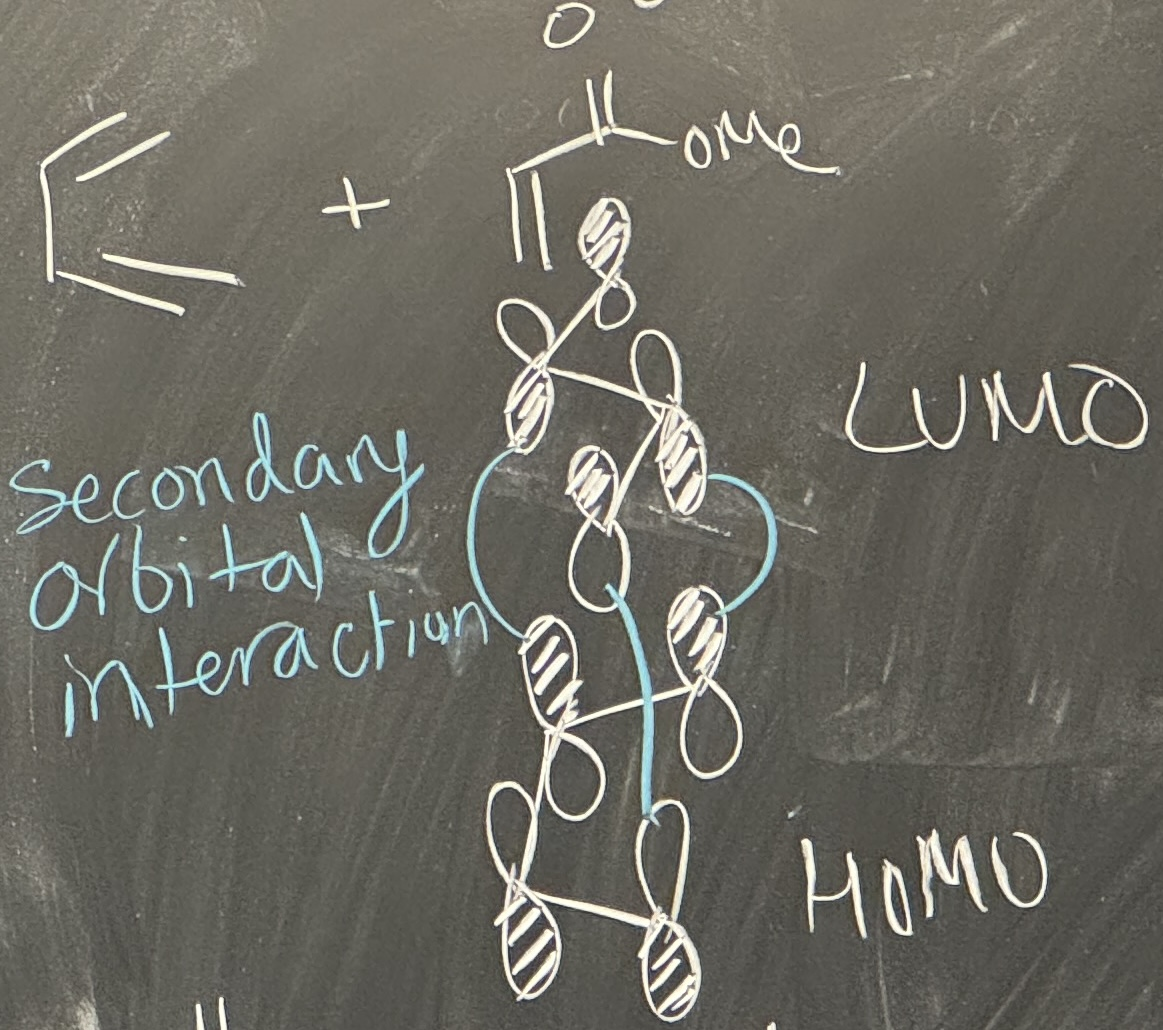
\includegraphics[width=0.76\linewidth]{FMOc.JPG}
            \caption{\emph{endo}-$[4+2]$.}
            \label{fig:FMOc}
        \end{subfigure}
        \caption{Frontier molecular orbital analysis of cycloadditions.}
        \label{fig:FMO}
    \end{figure}
    \begin{itemize}
        \item A $[2+2]$ cycloaddition (Figure \ref{fig:FMOa}).
        \begin{itemize}
            \item As in a Dewar-Zimmerman analysis we begin by drawing the HOMO and LUMO of the reactants and deciding the reaction topology.
            \begin{itemize}
                \item MOs: Recall that for ethene, the HOMO has 0 PIs and the LUMO has 1 PI.
                \item Topology: We have decided to have the `electron-donating' ethene attack from the bottom.
            \end{itemize}
            \item Then (also as in a Dewar-Zimmerman analysis) we connect lobes and check for bonding and antibonding interactions.
            \begin{itemize}
                \item Here, we have 1 bonding and 1 antibonding interaction.
            \end{itemize}
            \item The presence of an antibonding interaction means that this reaction is forbidden/disfavored.
            \item Bonus content: Ketenes engage in $[2+2]$ cycloadditions at ambient temperatures!
            \begin{itemize}
                \item Masha encourages us to look more into this!!
            \end{itemize}
        \end{itemize}
        \item A $[4+2]$ cycloaddition (Figure \ref{fig:FMOb}).
        \begin{itemize}
            \item Performing an analogous analysis to the above, we observe 2 bonding interactions. This means that this reaction is allowed.
        \end{itemize}
        \item A $[4+2]$ cycloaddition with a more elaborate dienophile (Figure \ref{fig:FMOc}).
        \begin{itemize}
            \item As in both previous cases, we begin by drawing the HOMO of the `electron-donating' species and the LUMO of the `electron-accepting' species.
            \begin{itemize}
                \item MOs: Notice that it does not matter that the dienophile's $\pi$-system contains a heteroatom.
                \item Topology: This time, we have the dienophile attack from the top.
            \end{itemize}
            \item Connecting orbitals.
            \begin{itemize}
                \item First, observe that we get the same favorable bonding interactions as in Figure \ref{fig:FMOb}.
                \item In addition, we get a new, secondary orbital interaction if we draw the \emph{endo} transition state.
                \item This additional, stabilizing interaction rationalizes why the \emph{endo} transition state is favored in a Diels-Alder reaction!
            \end{itemize}
            \item Therefore, this reaction is allowed, and the \emph{endo} product is preferred due to secondary orbital interactions.
        \end{itemize}
    \end{itemize}
    \item Miscellaneous pericyclics: Group transfer and chelotropic reactions.
    \item Recall from above that a \emph{group transfer} reaction transfers atoms from one molecule to another, but in a concerted pericyclic transition state.
    \item Example group transfer reactions.
    \begin{enumerate}
        \item \textbf{Diimide reduction}.
        \item The \textbf{ene reaction}.
    \end{enumerate}
    \item \textbf{Diimide reduction}: A group transfer reaction that converts an unsaturated organic compound to a reduced alkane using diimide (\ce{N2H2}).
    \begin{center}
        \footnotesize
        \setchemfig{atom sep=1.4em}
        \schemestart
            \chemfig[atom sep=2em]{*6([:-120]@{H1}H-[@{1}]N=[@{2}]N-[@{3}]@{H2}H)}
            \arrow{0}[,0.25]
            \chemfig{@{C2}=[@{4}2]@{C1}}
            \arrow
            \chemfig{N~[2]N}
            \arrow{0}[,0.1]\+{,,1.1em}
            \chemfig{*6([:60]H---H)}
        \schemestop
        \chemmove{
            % \draw [curved arrow={2pt}{4pt}] (3) to[bend right=60,looseness=1.5] (2);
            % \draw [curved arrow={2pt}{2pt}] (1) to[bend right=60,looseness=1.5] ($(H1)!0.5!(C1)$);
            % \draw [curved arrow={4pt}{2pt}] (4) to[bend right=60,looseness=1.5] ($(H2)!0.5!(C2)$);
            \draw [curved arrow={2pt}{4pt}] (1) to[bend left=60,looseness=1.5] (2);
            \draw [curved arrow={2pt}{2pt}] (3) to[bend left=60,looseness=1.5] ($(H2)!0.5!(C2)$);
            \draw [curved arrow={4pt}{2pt}] (4) to[bend left=60,looseness=1.5] ($(H1)!0.5!(C1)$);
        }
    \end{center}
    \begin{itemize}
        \item Remember to draw arrows to the place where you're making the bond, not to an atom unless the electrons are going on that atom!!
    \end{itemize}
    \item \textbf{Ene reaction}: A group transfer reaction between an \textbf{ene} and an \textbf{enophile} that forms a new $\sigma$-bond with migration of the ene double bond and a $1,5$-hydrogen shift. \emph{Also known as} \textbf{Alder-ene reaction}.
    \begin{center}
        \footnotesize
        \setchemfig{atom sep=1.4em}
        \schemestart
            \chemfig[atom sep=2em]{*6([:-120]@{H1}H-[@{1}]-[@{2}]=[@{3}]@{H2})}
            \arrow{0}[,0.25]
            \chemfig{@{C2}=[@{4}2]@{C1}}
            \arrow
            \chemfig{*6([:-60]=----H)}
        \schemestop
        \chemmove{
            \draw [curved arrow={2pt}{2pt}] (1) to[bend left=60,looseness=1.5] (2);
            \draw [curved arrow={4pt}{2pt}] (3) to[bend left=60,looseness=1.5] ($(H2)!0.5!(C2)$);
            \draw [curved arrow={4pt}{2pt}] (4) to[bend left=60,looseness=1.5] ($(H1)!0.5!(C1)$);
        }
    \end{center}
    \item \textbf{Ene}: An alkene with an allylic hydrogen.
    \item \textbf{Enophile}: A compound containing a multiple bond.
    \item Moving on, recall from above that a \emph{chelotropic} reaction is a cycloaddition in which two bonds are made to one atom.
    \item Example chelotropic reactions.
    \begin{enumerate}
        \item \textbf{Carbene addition}.
        \item Certain \textbf{cycloreversions}.
    \end{enumerate}
    \item \textbf{Carbene addition}: The addition of a singlet carbene to an alkene to make a cyclopropane.
    \begin{center}
        \footnotesize
        \setchemfig{atom sep=1.4em}
        \schemestart
            \chemfig{@{C1}=[@{1}2]@{C2}}
            \arrow{0}[,0.5]
            \chemfig{R-[:120]@{C3}\charge{180=\:}{}-[:60]R}
            \arrow
            \chemfig{*3(-(-[:20]R)(-[:-20]R)--)}
        \schemestop
        \chemmove{
            \draw [curved arrow={3pt}{0pt}] (1) to[bend left=30,looseness=1.5] ($(C1)!0.5!(C3)$);
            \draw [curved arrow={5pt}{0pt}] (C3) to[bend left=30,looseness=1.5] ($(C3)!0.5!(C2)$);
        }
    \end{center}
    \begin{itemize}
        \item Observe how the two arrows form two $\sigma$-bonds to the carbene.
    \end{itemize}
    \item \textbf{Cycloreversion}: The reverse of a cycloaddition reaction.
    \begin{center}
        \footnotesize
        \setchemfig{atom sep=1.4em}
        \setcharge{extra sep=5pt}
        \schemestart
            \chemfig[atom sep=2em]{*5(-[@{1}]-[@{2}]@{N1}\charge{90=$\oplus$}{N}(=[@{2a}]@{N2}\charge{90=$\ominus$}{N})-[@{3}]-[@{4}]=[@{5}])}
            \arrow
            \chemfig{*6([:-120]=-=)}
            \arrow{0}[,0.1]\+
            \chemfig{N~N}
        \schemestop
        \chemmove{
            \draw [curved arrow={4pt}{2pt}] (5) to[bend left=54,looseness=1.5] (1);
            \draw [curved arrow={2pt}{2pt}] (3) to[bend left=54,looseness=1.5] (4);
            \draw [curved arrow={10pt}{3pt}] (N2) to[bend right=90,looseness=3.5] (2a);
            \draw [curved arrow={2pt}{1pt}] (2) to[bend right=60,looseness=2] (N1);
        }
    \end{center}
    \begin{itemize}
        \item Since two of the left nitrogen's bonds are being \emph{broken}, this is technically a \emph{retro-chelotropic} reaction.
    \end{itemize}
    \pagebreak
    \item Lecture summary: Three models to study pericyclic reactions.
    \begin{enumerate}
        \item The Woodward-Hoffmann rules.
        \begin{itemize}
            \item These are all about the conservation of orbital symmetry.
        \end{itemize}
        \item The Dewar-Zimmerman analysis, also known as aromatic TS theory.
        \begin{itemize}
            \item This is the "I can't believe it works!" one, where you can draw any phasing and the model still gives you the right answer.
        \end{itemize}
        \item FMO theory.
        \begin{itemize}
            \item This is where we only look at HOMO/LUMO interactions.
        \end{itemize}
    \end{enumerate}
    \item Matthew: When would you use one model over the others?
    \begin{itemize}
        \item All three models should always give the same result (otherwise, there's a problem with the model), but sometimes you care more about one aspect of a reaction or another.
        \item For example, if you want to figure out whether you get the conrotatory or disrotatory product, it is easier to use the Woodward-Hoffmann rules.
        \begin{itemize}
            \item This is because they're designed specifically for such questions.
        \end{itemize}
        \item If you need a quick-and-dirty "is this reaction going to happen," use FMO.
        \item If you want to determine whether a reaction will be antarafacial or suprafacial, use Dewar-Zimmerman.
    \end{itemize}
\end{itemize}



\section{Chapter 14: Advanced Concepts in Electronic Structure Theory}
\emph{From \textcite{bib:Anslyn}.}
\subsection*{Section 14.2: Calculational Methods --- Solving the Schr\"{o}dinger Equation for Complex Systems}
\begin{itemize}
    \item \marginnote{9/23:}20 pages on computational methods, but a bit outdated.
\end{itemize}



\section{Chapter 15: Thermal Pericyclic Reactions}
\emph{From \textcite{bib:Anslyn}.}
\begin{itemize}
    \item This whole chapter is a gold mine. Return to!!
\end{itemize}


\subsection*{Section 15.1: Background}
\begin{itemize}
    \item 
\end{itemize}


\subsection*{Section 15.2: A Detailed Analysis of Two Simple Cycloadditions}
\begin{itemize}
    \item 
\end{itemize}


\subsection*{Section 15.3: Cycloadditions}
\begin{itemize}
    \item 
\end{itemize}


\subsection*{Section 15.4: Electrocyclic Reactions}
\begin{itemize}
    \item 
\end{itemize}


\subsection*{Section 15.5: Sigmatropic Rearrangements}
\begin{itemize}
    \item 
\end{itemize}



\section{Chapter 16: Photochemistry}
\emph{From \textcite{bib:Anslyn}.}
\begin{itemize}
    \item Also a treasure trove, though much of this is beyond the scope of the course. However, it is largely within the scope of 5.47, so I should definitely return!!
\end{itemize}


\subsection*{Section 16.3: Photochemical Reactions}
\begin{itemize}
    \item Recommended readings for this course: Sections 16.3.4-16.3.5.
    \item The tail-end of 16.3.5 talks a bit about norbornadiene (PSet 1).
\end{itemize}




\end{document}